\documentclass[12pt]{article}

\usepackage{fullpage}
\usepackage{graphicx}
\usepackage{graphics}
\usepackage{mdwlist}
\usepackage{listings}
\usepackage{caption}
\usepackage{subcaption}
\usepackage{subfig}

\usepackage[ruled,vlined,linesnumbered]{algorithm2e}


% christos: these look closer to NSF specs\dots
\setlength{\oddsidemargin}{0.0in}
\setlength{\evensidemargin}{0.0in}
\setlength{\textwidth}{6.5in}
\setlength{\headheight}{0.0in}
\setlength{\topmargin}{0.0in}
% \setlength{\textheight}{9.0in}
\setlength{\textheight}{9in}
\addtolength{\textheight}{-\topmargin}
\addtolength{\textheight}{-\headheight}
\addtolength{\textheight}{-\headsep}
\addtolength{\textheight}{-\footskip}



\begin{document}

\newcommand{\beq}{\begin{equation}}
\newcommand{\eeq}{\end{equation}}
\newcommand{\bit}{\begin{itemize*}}
\newcommand{\eit}{\end{itemize*}}
\newcommand{\goal}[1]{ {\noindent {$\Rightarrow$} \em {#1} } }
\newcommand{\hide}[1]{}
\newcommand{\comment}[1]{ {\footnotesize {#1} } }
\newtheorem{lemma}{Lemma}
\newtheorem{theorem}{Theorem}
\newtheorem{proof}{Proof}
\newtheorem{defn}{Definition}
\newtheorem{algo}{Algorithm}
\newtheorem{observation}{Observation}

\title{Carnegie Mellon University \\
15-826 Multimedia Databases and Data Mining \\
Fall 2013 - C. Faloutsos \\
Project 2: Graph Mining using SQL \\
Final Report}


\author{ {\em Emma R. Zhang} \\
	    School of Computer Science \\
	    {\tt runyunz@andrew.cmu.edu(runyunz)}
	 \and
	 {\em Fangyu Gao} \\
	      School of Computer Science \\
	      {\tt fangyug@andrew.cmu.edu(fangyug)}
        }


\maketitle
\begin{abstract}
    It is natural to expect performing data mining in RDBMS, where data stored.
Can we perform graph mining directly in database, without moving data all round?
Can we implement various graph query methods via SQL, so as to leverage the powerful support from RDBMS?
Can we figure out a maverick graph, which has unusual features among a similar set of graph datasets?
In this project, our goal is to implement a SQL version of graph mining algorithms, and perform broad spectrum graph mining on a variety of graph dataset with the support of RDBMS.  


\end{abstract}

\section{Introduction}
    \label{sec:intro}
    % {\em
% \bit
% \item
% what is the problem
% \item
% what are the applications
% \eit
% }
% {\small \em Specify the problem; Give the motivation; 
% List your main contributions}

The problem we want to solve is the following:
\bit
\item GIVEN: a collection of graph datasets from various scenarios
\item FIND: 'strange' datasets which have different behaviors versus the majority datasets
\item to IMPLEMENT: a set of powerful graph mining methods in SQL on RDBMS, including {\em degree distribution, page rank, connected components, radius, eigenvalues/singular values, Belief Propagation, Count of Triangles, etc.}
\eit

Data, especially those containing valuable information, are stored in Database. Therefore, it is reasonable that people wish to perform data mining directly within RDBMS. In addition, RDBMS offers powerful support from all perspective, be it sophisticated data management mechanism, fine-tuned query optimization, and easy-to-use interface language: SQL. However, the challenge is that it is a unnatural way to implement graph query algorithms using ralational query. Therefore, our goal is to address this problem so that we can perform graph mining with full support of RDMS and find interesting patterns of various graph datasets. 

The contributions of this project are the following:
\bit
\item Our implementation of graph queries algorithms in SQL provide a native way for graph mining to take advantage of RDBMS
\item Based on our implementated algorithm, we can perform broad spectrum graph mining on a variety of graph dataset efficiently
\eit


\section{Survey}
    \label{sec:survey}
    Next we list the papers that each member read,
along with their summary and critique.
Table \ref{tab:symbols} gives a list of common symbols we used.

\begin{table}[htb]
\begin{center} 
\begin{tabular}{|l | c | } \hline \hline 
Symbol & Definition \\ \hline
$V$ & Vertices of graph \\
$E$ & Edges of graph \\ \hline
\end{tabular} 
\end{center} 
\caption{Symbols and definitions}
\label{tab:symbols} 
 \end{table} 


\subsection{Papers read by Emma Zhang}
The first paper was the GBASE paper \cite{KangTSLF12}.
\begin{itemize*}
\item {\em Main idea}: 
	  GBASE is a efficient, scalable platform on Hadoop designed for large-scale graph mining(e.g. perform real analysis on YahooWeb, one of the largest graphs in the world with 1.4 billion nodes, 6.6 bilion edges and 120GB in space). 
	  
	  The overall framework of GBASE is composed of two stages. 
	  During the indexing stage, GBASE offers a novel graph storage method. By using a set of carefully-designed clustering, compression and blocking algorithms, the new method enjoys high performance in terms of space efficiency, running time, and machine scalability. 

	  During the query stage, GBASE unifies 11 types of graph query operations by matrix-vetor multiplication, including {\em degree distribution, PageRank, Random Walk with Restart, radius estimations, discovery of connected components, LineRank} as global queries, and {\em neighborhod, induced subgraph, Egonet, K-core, cross-edges and single source shortest distances as targeted queries}. Compared with previous work(PEGASUS \cite{KangTF11}), the contribution of GBASE is that 1) node-based and edge-based queries are unified; 2) the platform supports both adjacency matrix and incidence matrix. 
	  
	  In a nutshell, GBASE solves problem and achieves remarkable improvement in terms of storage, algorithms and query optimization. 
\item {\em Use for our project}:
      In addition to the Matrix-Vector implementation on Hadoop, the author also provided the SQL version of code for targeted queries.He also points out that matrix-vector multiplication naturally corresponds to SQL join, and implementing graph mining with SQL could benefit a lot from DBMS (e.g. using optimized join alorithms). 

      As for our project, we can refer to the SQL code that the paper provides and implement more queries such as {\em neighbors, induced subgraph, egonet,} etc.
\item {\em Shortcomings}:
      Since GBASE is built on Hadoop, the paper does not mention how graph queries performs on RDBMS. Also, as the SQL version of global graph queries({\em degree distribution, PageRank}, etc.) are not covered.
\end{itemize*}

The second paper was the HADI paper \cite{Kang:2011:HMR:1921632.1921634}.
\begin{itemize*}
\item {\em Main idea}:
	   HADI(HAdoop DIameter and radii estimator) is used for computing the radii and the diameter of Petabyte-scale graphs. To compute effecitive radius and diameter in a efficient way, HADI is designed as an approximation algorithm running on parallel platform like Hadoop, and also can be adapted to parallel RDBMS. Specially, Flajolet-Martin algorithm [Flajolet and Martin 1985; Palmer et al. 2002] is adopted for counting the number of distinct elements in a multiset for its unbiased estimation and linear time performance.

	   The paper then discusses the detailed implementation and optimization of HADI on Hadoop. It also explores a little on how to adapt HADI to RDBMS system and provides a sketch of potential implementation of HADI using SQL.

	   Finally, by applying HADI to mining massive real graph(YahooWeb, Twitter, etc.), the author successfully observes and reports several interesting patterns on large networks. 
\item {\em Use for our project}:
	   One insight the paper gives is that using RDBMS for graph mining tend to be a promising direction, becuase RDBMS has a couple of advantages versus Hadoop(e.g. performance)\cite{pavlo09}. 

	   Also, the paper provides a solution of implementing HADI in SQL through repeated joins of edge table, as well as a unser-defined function of related operations(bit-OR in this case). This could be a good start point for us to complete the radius query task.
\item {\em Shortcomings}:
       Similar to GBASE paper, HADI is fine-tuned for Hadoop platform. Therefore, for diameter/radius estimation we can explore other methods in addition to HADI which might work better on RDBMS.      
\end{itemize*}

The third paper was the FABP paper \cite{koutra2011unifying}.
\begin{itemize*}
\item {\em Main idea}:
	   The paper analizes three successful methods on Guilt-by-Association: {\em Random Walk with Restarts(RWR), Semi-supervised Learning(SSL), and Belief Propagation(BP)}, and shows that all of them can be viewed as a matrix inversion problem. According to the paper, Belief propagation is recommended among three methods for its solid Bayesian basis as well as capability to deal with heterophily and multiple class-lable.

	   The author then proposes FABP, an approxmimation method of standard BP, followed by a series of analyses and experiments indicating its advtanges in terms of performance, accuracy and scalability. 
\item {\em Use for our project}:
	   The paper provided comprensive analyses on BP and other userful graph mining algorithms like RWR. It also gives sound proof of the FABP algorithm so that we can follow its step to implement a fast BP variant on RDBMS.

	   In addition to this paper, the paper \cite{KangCF11} also provide insights for the BP algorithm because it shares consisten implementation with the PEGASUS \cite{KangTF11} paper. 
\item {\em Shortcomings}:
       Although the paper implements FABP on hadoop and show it works very well, it does not expend effort on RDBMS implementation. We need to figure out a SQL version of code based on the general description of algorithm, and see how FABP works on RDBMS.		
\end{itemize*}

The forth paper was the benchmark paper by A. Pavlo \cite{pavlo09}.
\begin{itemize*}
\item {\em Main idea}:
	   The paper focus on large-scale data analysis. After profound study on the architecture design of parallel DBMS and Map Reduce, the author defines and performs a comprensive benchmark test to support the earlier conclusions about the pros and cons of DBMS versus Map Reduce. 

	   The paper compares MapReduce frame with DBMS from 7 perspectives: {\em schema support, indexing, programming model, data distribution, execution strategy, flexibility, and fault tolerance}. As for the real experiment, Haddop, a column-store DBMS and a traditional row-store DBMS are used for benchmark tests. The tests includes data processing tasks(the original Map Reduce task) and analytical tasks(Data Loading, Selection, Aggregation, Join, and UDF aggregation). 

	   Combining theory analysis and experiment results, the paper concludes that parallel DBMS has its advantages that Map Reduce platform cannot replace, and future systems should take insights from both kinds of architectures.
\item {\em Use for our project}:
	   The paper bring up several insights to our project. First, it is promising to perform data mining within RDBMS. Second, column-store analytical DBMS worths our notice. Third, it shows how to rewrite Map Reduce programming paradigm with SQL using UDF. Finally, we can learn a lot from the benchmark test part when performing our analysis. 
\item {\em Shortcomings}:
       One fact the paper does not bring about is most of powerful parallel DBMS are commercial, while Hadoop is open-sourced and free,
       which contribute to an important reason why people tend to use Hadoop for large-scale data mining.
\end{itemize*}

\subsection{Papers read by Fangyu Gao}
The first paper was the PEGASUS paper \cite{KangTF11}.
\begin{itemize*}
\item {\em Main idea}:
	   It describes why data mining in large graph is inevitable, and has to rely on MapReduce and HADOOP framework to implement large scale algorithms.

       The author unifies a bunch of algorithms in a GIM-V (Generalized Iterative Matrix-Vector multiplication) primitive, making seemly unrelated algorithms like PageRank, Random Walk, Diameter Estimation, Connected Components, etc. have a uniform abstraction. 

       Using the GIM-V primitive, the author easily transferred the algorithms to the HADOOP framework. Moreover, some optimization methods can be applied on HADOOP, including Block Multiplication, which brings less number to sort and data compression, Clustered Edges, which we can reuse the preprocessing result for edge clustering for various applications, Diagonal Block Iteration, which decrease the number of iterations, Node Renumbering, which swapped minimum node id o the center node id. The author proofs that the time complexity of GIM-V is $O(\frac{V+E}{M}log\frac{V+E}{M})$, while the space complexity is $O(V+E)$.

       In the end, the author did experiments to show that all of the basic graph mining methods listed above are doing well, and some interesting discovers like power law of large scale datasets can be found thanks to the new technique.
\item {\em Use for our project}:
	   This paper introduces to me what graph mining can do. By searching new terminologies appears in this paper, I become to understand the goal of my whole project. Moreover, it provides me with the framework and basic methods to do graph mining in SQL.Furthermore, it equipped me with powerful optimization method I can use when facing large datasets.
\item {\em Shortcomings}:
       Some trivial problems exists in the paper such as the meaning of some variables were not made clear (e.g. $x$ in the {\em combineAll} from the same space). 
\end{itemize*}

The second paper was the HEIGN paper \cite{KangMF12}.
\begin{itemize*}
\item {\em Main idea}:
	   The eigenvalues and eigenvectors are the basic of many algorithms, but existing algorithms calculating these don’t scale well on large dataset. And even billion-scale graphs are common nowadays like data from websites.

	   This paper describes a method called HEigen that calculate the first several eigenvalues and eigenvectors of graph adjacency matrix and run on the MapReduce environment.

	   Using this algorithm enabled the author to mining in large scale data, and discovered many important observations from large graph data. For example, spotting near cliques, triangle counting and eigen exponent.

	   Although there are many eigensolvers commonly used when dataset is small, none of them is easily scalable to calculate more than one eigenvalue and eigenvector in very large dataset. The power method computes only the first eigenvector, QR algorithm is expensive due to using matrix-matrix multiplication, Lanczos-NO method outputs spurious eigenvalues because of rounding error.

	   The author chose Lanczos-SO method that overcome all these shortcomings, and farther proposed parallelizing and a serial of optimization that make the algorithm run very fast on HADOOP. 
\item {\em Use for our project}:
	   This paper helps me review some basic mathematical knowledge for me to complete task 5 of project 2. It also teaches me some useful optimization method to work on big data.
\item {\em Shortcomings}:
       The algorithm is only applicable to symmetric matrix, so it can only calculate eigenvalues and eigenvectors of undirected-graphs.
\end{itemize*}

The third paper was about Fast Couting of Triangles \cite{4781156}.
\begin{itemize*}
\item {\em Main idea}:
	   This paper proposed ways to fast counting of triangles in large real networks by a high accuracy way. The author used the method to count the triangles of the whole graph as well as count the triangles of a single node, which is very useful especially in social network.

	   The paper introduces some non-streaming algorithms, like Brute-Force, Edge Iterator and Node Iterator, to count the number triangles in a graph exactly. Without any exception, these methods all have high computational complexity. Then, the author turns to streaming algorithms, but most of the works lack proof and justification.

	   Therefore, before proposing the method, the author gives proof of the theorems he uses, including Eigen Triangle and Local Eigen Triangle. Then the proposed algorithms based on Lanczos method is given, and the author explains why the method is successful in real-world networks. 

	   Based on the fast and successful experimental results he gets, the author discovers new power laws, the Triangle Participation law and Degree-Triangle law. 
\item {\em Use for our project}:
	   By learning the counting of triangles in a graph, I gain better intuitive understanding of eigenvalues and eigenvectors. The paper makes me understand why some proximate algorithms could get very high accuracy, which could help me choose the testing dataset in the project. According to the exact algorithms introduces in the paper, we could choose the most fast one for grand truth of our testing.
\item {\em Shortcomings}:
       The author implements the algorithm in MATLAB. This does not mean that the algorithm will still working well in MapReduce. To proof the algorithm is robust in large scale using MapReduce, the author needs to do more experiment.
\end{itemize*}


\section{Proposed Method}
    \label{sec:proposed}
    \subsection{Task List}
Our goal is to implement as many tasks from the task list as possible, apply them on as many of the datasets as applicable, and study the results.

The task list includes following tasks:
\bit
\item Task 1: Degree distribution
\item Task 2: PageRank
\item Task 3: Connected components
\item Task 4: Radius and Diameter
\item Task 5: Eigenvalues
\item Task 6: Belief Propagation
\item Task 7: Count of Triangles
\item Innovation Tasks: Directed, Undirected, and Weighted Graph
\eit

\subsection{Implementation Choice}
We use PL/pgSQL for implementation. PL/pgSQL is the procedural language for the PostgreSQL database system. PL/pgSQL extends the functions of SQL by adding control structures(e.g. condition and loop), and thus supporting complex computations. \\
We consider implementing User-defined Functions(UDFs) and Stored Procedures(SPs) using SQL and register them in the DBMS server, which is a good practice for traditional OLTP to improve performance. For OLAP system and data mining tasks, though communication cost is no longer the main concern, maintaining a ready-to-use data mining package at DB server is still helpful to make data analysis easier. \\
Another reason for choosing PL/pgSQL that is is native to the DB system. PL/pgSQL inherits all user-defined types, functions, and operators from PostgreSQL, so that we can take advantage of the powerful feature of DBMS system itself. 

\subsection{Basic Operation}
According to the Pegasus paper\cite{KangTF11}, most of the tasks can be represented as performing iterations on a generalized matrix-vector multiplication. Listing \ref{gc} gives the SQL code of this general implementation:
\begin{lstlisting}[caption=General Procedure, label=gc, language=SQL, numbers=left, numberstyle=\tiny, breaklines, tabsize=2, frame=single]
	UPDATE vector
	SET val = new_vector.val FROM
	(SELECT matrix.row, aggregate(matrix.val*vector.val)
		FROM matrix, vector
		WHERE matrix.col = vector.row
		GROUP BY matrix.row) new_vector
	WHERE vector.row = new_vector.row
\end{lstlisting}
In addition, we find it useful to implement a set of basic operations separately for code re-usability. For example, UDF $node\_lst$ is used for multiple times to compute the node list given the edge list.
\begin{verbatim}
	INSERT INTO node_lst
		SELECT n_from AS node FROM adj_lst 
		UNION DISTINCT 
		SELECT n_to AS node FROM adj_lst ORDER BY node;
\end{verbatim}

\subsection{Task 1: Degree Distribution}
\subsubsection{Method Description}
The major work for degree distribution task contains two steps. First, count the degree for each node(both in-degree and out-degree for directed graph). Second, for data visualization purpose(i.e. to discover power law distribution), we perform a following data processing step to count and calculate the number of nodes having the same in/out-degree. \\

\subsubsection{SQL Implementation}
We give the SQL implementation as follows:
\begin{lstlisting}[caption=Degree Distribution, label=dd, language=SQL, numbers=left, numberstyle=\tiny, breaklines, tabsize=2, frame=single, keepspaces=false]
	CREATE degree
		SELECT node, count(node) AS degree 
		FROM edge_lst 
		GROUP BY node;
	SELECT degree, count(*) AS count 
	FROM degree
	GROUP BY degree;
\end{lstlisting}

\subsection{Task 2: PageRank}
\subsubsection{Method Description}
The famous PageRank algorithm is originally invented by Google for search result ordering. The algorithm ranks web pages by adopting the rule that a web page having a lot of important web pages link to will also get a high score. \\
Using the power method, the algorithm can be described as iteratively multiplication on rank vector by adjacency matrix. Considering the damping points(points with no out-degree) cases, we introduce the damping factor $d$(by default \(d=0.85\)) to enable fly-out. With probability \(1-d\), random walk will fly out randomly to a new node.\\
The equation of PageRank can be represented as follows:
\[M=dA^T + \frac{1-d}{N}I,\ p=Mp\]
where $p$ is the PageRank vector, $A$ is the normalized adjacency matrix(i.e. \(\sum(row) = 1\)), and $d$ is the damping factor.\\
Considering the scalability of the algorithm, we take advantage of the sparcity of matrix and computing with only the edges in the adjacency list.Concretely, we compute \[p_{next} = Mp_{now} = dA^Tp_{now} + \frac{1-d}{N}\mathbf{1}^Tp_{now}\] every iteration, rather than building up the full matrix and add constant to every elements at first time. \\
We provide algorithm \ref{pr} for a brief description.
\begin{algorithm}[htbp]
	\SetAlgoLined
	load data in adjacency list\;
	build up transposed adjacency matrix $A^T$ given the adjacency list\;
	initilize PageRank vector $V$\;
	\For{$i\leftarrow 1$ \KwTo $n$}{
	update $p$ with \(dA^Tp_{now} + \frac{1-d}{N}\sum{p_{now}}\)\;}
	\caption{PageRank}
	\label{pr}
\end{algorithm}

\subsubsection{SQL Implementation}
To compute PageRank, we first need a intialized rank vector setting every node to the uniform distribution probability(1/count of node).
We implement User-Defined Function $pr\_rank$ to perform the job.
\begin{verbatim}
	EXECUTE 
	'SELECT CAST(1 AS double precision)/count(*) 
	FROM node_lst' INTO n;

	EXECUTE
	'INSERT INTO pr_rank 
		SELECT node AS v_row, $1 AS v_val 
		FROM node_lst' USING n;
\end{verbatim}
Second, we compute the normalized transposed adjacency matrix $A^T$ using UDF $adj\_matrix\_trans$.
\begin{verbatim}
INSERT INTO adj_matrix 
	SELECT n_to AS m_row, n_from AS m_col, 
		CAST(1 as double precision)/degree.degree AS m_val 
	FROM adj_lst, degree
	WHERE adj_lst_weighted.n_from = degree_weighted.node;
\end{verbatim}
Then we update the PageRank iteratively as follows. The first EXECUTE clause compute the constant and the second EXECUTE perform the general procedure of matrix-vertex multiplication.
\begin{lstlisting}[caption=PageRank, label=pr, language=SQL, numbers=left, numberstyle=\tiny, breaklines, tabsize=2, frame=single, keepspaces=false]
	EXECUTE 'SELECT count(*) FROM node_lst' INTO n;
	
	FOR i IN 1..iter LOOP
		EXECUTE 'SELECT SUM(v_val) * (1 - $1)/$2 FROM pr' INTO y USING d, n;
		EXECUTE
		'UPDATE pr
		SET v_val = $1 * p1.v_val + $2 FROM 
			(SELECT adj_matrix.m_row AS v_row, SUM(adj_matrix.m_val * pr.v_val) AS v_val
			FROM adj_matrix, pr
			WHERE adj_matrix.m_col = pr.v_row
			GROUP BY adj_matrix.m_row) p1
		WHERE pr.v_row = p1.v_row' USING d, y;
	END LOOP;
\end{lstlisting}

\subsection{Task 3: Connected Component}
\subsubsection{Method Description}
The main idea of Connected Component is that each node maintains and updates its connected component among the connected components from its neighbors. \\
To start with, we set the connected component to each node itself. For each iteration, every node receive a list of connected components from its neighbor node, then it pick the smallest node id from the list as well as its current connected component, and keep that node id as the new connected component. \\
The algorithm is described as follows.
\begin{algorithm}[htbp]
	\SetAlgoLined
	load data into adjacency list $E$\;
	create the connected component list $C$\;
	initialize $C$ by setting connected component to each node itself\;
	\For{$i\leftarrow 1$ \KwTo $n$}{
		\(C(i) = min(C(i), C_{(i,j) \in E}(C(j))\)\;}
	\caption{Connected Component}
	\label{cc}
\end{algorithm}

\subsubsection{SQL Implementation}
The main body of connected component algorithm is also a varient of basic operation, where the minumum function serve as the aggregate function.
\begin{lstlisting}[caption=Connected Component, label=cc, language=SQL, numbers=left, numberstyle=\tiny, breaklines, tabsize=2, frame=single, keepspaces=false]
	UPDATE conn_comp
	SET comp = n1.comp FROM 
		(SELECT adj_lst.n_from AS node, MIN(conn_comp.comp) AS comp
		FROM adj_lst, conn_comp
		WHERE adj_lst.n_to = conn_comp.node
		GROUP BY adj_lst.n_from) n1
	WHERE conn_comp.node = n1.node;
\end{lstlisting}
In addition, we also keep track of the size of Global Connected Component(GCC). In this way, we are able to stop the iteration once its value stops changing. \\
Here are the detailed implementation:
\begin{verbatim}
	EXECUTE 
	'SELECT count(*) AS gcc_count 
	FROM conn_comp 
	GROUP BY comp 
	ORDER BY gcc_count DESC 
	LIMIT 1' INTO gcc_count;

	IF gcc_count = gcc_last THEN
		EXIT;
	END IF;

	EXECUTE 
	'INSERT INTO comp_track VALUES($1, $2)' USING i, gcc_count;

	gcc_last = gcc_count;
\end{verbatim}

\subsection{Task 4: Radius}
\subsubsection{Method Description}
In this case, we refer to HADI algorithm\cite{Kang:2011:HMR:1921632.1921634}. Concretely, we first set up 32 Flajolet-Martin bit string of length 32 for each node. Flajolet-Martin algorithm\cite{Flajolet:1985:PCA:5212.5215} approximates the number of unique objects in a stream or a database in one pass. Then during every iteration, we perform bit-wise OR among the bit-string list of the node together with the bit-string list of its neighbors. \\
We maintain a copy of the bit-string list to keep track of the result. As long as the bit-string for a node stops changing, we insert that node to the radius list with its radius as the number of current iteration. And we stop tracking that node by deleting it from the check list. If the check list is empty, then we finish the looping and check the radius list. All the nodes are supposed to be in the list now. And the maximum radius in the list will serve as the diameter of the whole graph.\\
To simplify the process, we add a self-loop for each node(i.e. input all (i, i) into edge list), which means we can perform bit-wise operation directly on the query result on neighbor nodes from edge list. \\
In algorithm \ref{rd}, we provide detailed description in terms of pseudo code.
\begin{algorithm}[htbp]
	\SetAlgoLined
	load data into adjacency list\;
	create and initialize the fm\_bit string list for each node\;
	create and initialize the check list from bit string list\;
	create the radius list\;
	\While{check list is not empty}{
		perform bit-or operation on the bit string list of the node and its neighbors\;
		\If{the new bit string = the old bit string}
			{
				add the node into the radius list\;
				remove the node from the check list\;
			} 
		update the check list with the new bit strings\;
		}
	diameter = max(radius list)\;
	\caption{Radius and Diameter}
	\label{rd}
\end{algorithm}

\subsubsection{SQL Implementation}
The first thing we do is to add self-loop via UDF $self\_loop$.
\begin{verbatim}
	INSERT INTO adj_lst 
		SELECT node as n_from, node as n_to FROM node_lst;
\end{verbatim}
After that, we generate the 32 Flajolet-Martin bit string list for each node.
\begin{verbatim}
	FOR i IN 1..n LOOP
		FOR j IN 1..32 LOOP
			arr[j] := 2 ^ floor(random()*32);
		END LOOP;
		EXECUTE 'INSERT INTO bit_str VALUES($1, $2)' using CAST(i as bigint), arr;
	END LOOP;
\end{verbatim}
Then we use the basic operation to update the bit string for each node using Bit-OR function as the aggregate funciton, which is provided by postgres here.
\begin{lstlisting}[caption=Radius, label=rd, language=SQL, numbers=left, numberstyle=\tiny, breaklines, tabsize=2, frame=single, keepspaces=false]
	UPDATE bit_str
	SET str = str_new.str
	FROM(
		SELECT adj_lst.n_from AS n_from, bit_or(bit_str.str)
		FROM adj_lst, bit_str
		WHERE adj_lst.n_to = bit_str.node
		GROUP BY adj_lst.n_from) str_new
	WHERE bit_str.node = str_new.n_from;
\end{lstlisting}
Finally, we repeat the process of removing stable node from check list and stop the iteration until the list is empty.
\begin{verbatim}
	TRUNCATE temp;
	INSERT INTO temp
		SELECT bit_str_check.node FROM bit_str_check, bit_str 
			WHERE bit_str_check.node = bit_str.node AND bit_str_check.str=bit_str.str;

		EXECUTE 'INSERT INTO node_radius (SELECT node, $1 FROM temp)' using round;

		DELETE FROM bit_str_check WHERE node IN 
		(SELECT node FROM temp);

	SELECT COUNT(*) FROM bit_str_check into count;
	IF count = 0 THEN
		EXIT;
	END IF;

	UPDATE bit_str_check 
	SET str=bit_str.str
	FROM bit_str
	WHERE bit_str_check.node = bit_str.node;
\end{verbatim}


\subsection{Task 5: Eigenvalues}
\subsubsection{Method Description}
We implemented the Lanczos-NO algorithm in the paper “HEigen: Spectral Analysis for Billion-Scale Graphs”\cite{KangMF12}, the algorithm is described as follows.\\
\begin{algorithm}[htbp]
	\SetAlgoLined
	generate a vector with size equal to the column number of adjacency matrix; let it be the initial base $v_i$\;
	\For{$i\leftarrow 1$ \KwTo $n$}{
		Find a new basis vector\;
		Orthogonalize against two previous  basis vectors\;
		build tri-diagonal matrix\;
		Eigen decomposition of the tri-diagonal matrix\;
		selectively re-orthogonalize the new basis vector\;
		}
	build the last tri-diagonal matrix\;
	Eigen decompose the last tri-diagonal matrix\;
	compute the top k diagonal elements\;
	compute eigenvectors\;
	\caption{Eigenvalues}
	\label{ev}
\end{algorithm}

\subsubsection{SQL Implementation}
Most of the operations in this task are matrix multiplications and vector multiplication. The implement of these are the same as before. 
\lstinputlisting[caption=Eigenvalues, language=SQL, numbers=left, numberstyle=\tiny, breaklines, tabsize=2, frame=single]{CODE/eigen.sql}

\subsection{Task 6: Belief Propagation}
\subsubsection{Method Description}
Belief Propagation is a commonly-used message passing algorithm to perform inference on graphical model, such as Bayesian networks(directed graph) and Markov random fields(undirected graph). \\
As for algorithm, we implemented FastBP\cite{koutra2011unifying}, a fast approximate BP algorithm guaranteed to converge. The equation we refer to are as follows.
\[M=aD − c^{′}A,\ b^{t+1}=Mb^t,\ belief=\sum(b)\]
\[D=\sum_j{A_{ij}}\ and\ D_{ij}=0\ for\ i \ne j\]
\[c_1 = 2+\sum_i{d_{ii}},\ c_2=\sum_i{d_{ii}}^2-1,\ h_h < \sqrt{\frac{-c_1+\sqrt{c_1^2+4c_2}}{8c_2}}\]
\[a=\frac{4h_h^2}{1-4h_h^2},\ c^{'}=\frac{2h_h}{1-4h_h^2}\]
The implementation of Belief Propagation algorithm is similar to PageRank. We sum over the result of vector after each iteration to get the final approximate of belief for each node. Also, we ultilize the sparse matrix. Instead of generating the whole matrix, we only compute the elements in the edge list as well as on the diagonal, which means great news for large-scale graph mining. \\
The algorithm of FastBP is described as follows.
\begin{algorithm}[htbp]
	\SetAlgoLined
	load data into the adjacency list, which also serves as adjacency matrix $A$here\;
	load data into the initial belief list $b$\;
	create and compute trace matrix $D$ from $A$\;
	compute $c_1$, $c_2$, and $h_h$ using $D$\;
	compute $a$ and $c^{'}$ using $h_h$ \;
	scale $A$ and $D$ using $a$ and $-c^{'}$; union the result as the matrix $M$\;
	create final belief list $b_{final}$; initial it using $b$\;
	\While{$b_{final}$ does not converge}{
		update $b$ with $Mb$\;
		update $b_{final}$ by adding $b$\;
		}
	\caption{Belief Propagation}
	\label{bp}
\end{algorithm}

\subsubsection{SQL Implementation}
Before starting the inference process, we first compute the related parameters to be used.
\begin{verbatim}
	CREATE TABLE d_matrix AS
		SELECT m_row, m_row as m_col, SUM(m_val) as m_val from adj_matrix GROUP by m_row;

	EXECUTE 'SELECT SUM(m_val) + 2 from d_matrix' INTO c1; 
	EXECUTE 'SELECT SUM(m_val^2) - 1 from d_matrix' INTO c2; 

	hh = sqrt((-c1 + sqrt(c1 ^ 2 + 4 * c2)) / (8 * c2));
	a = 4 * (hh ^ 2) / (1 - 4 * (hh ^ 2));
	c_prime = 2 * hh / (1 - 4 * (hh ^ 2));

	EXECUTE 
	'CREATE TABLE w_matrix AS
		(SELECT m_row, m_col, $1 * m_val AS m_val FROM adj_matrix)
		UNION
		(SELECT m_row, m_col, $2 * m_val AS m_val FROM d_matrix)' USING a, (-c_prime);
\end{verbatim}
Then we create two vectors and initiazed them with the proir belief. After that, we kick off the iteration preocess. The main body of iteration follows the basic matrix-vector multiplication paradigm.
\begin{lstlisting}[caption=Belief Propagation, label=bp, language=SQL, numbers=left, numberstyle=\tiny, breaklines, tabsize=2, frame=single, keepspaces=false]
	UPDATE b_vector
	SET v_val = b_new.v_val
	FROM(
		SELECT m_row AS v_row, 
		SUM(m_val * b_vector.v_val) AS v_val
		FROM w_matrix, b_vector
		-- FROM adj_matrix, b_vector
		WHERE m_col = b_vector.v_row
		GROUP BY m_row) b_new
	WHERE b_vector.v_row = b_new.v_row;

	UPDATE belief
	SET v_val = belief.v_val + b_vector.v_val FROM b_vector
	WHERE belief.v_row = b_vector.v_row;	
\end{lstlisting}

\subsection{Task 7: Count of Triangles}
\subsubsection{Method Description}
We implemented the EigenTriangle function in the paper “Fast Counting of Triangles in Large Real Networks: Algorithms and Law”\cite{4781156}. \\
The paper proofs: The total number of triangles in a graph is proportional to the sum of cubes of eigenvalues.
\[\Delta(G) = \frac{1}{6}\sum_{i=1}^n{\lambda^3}\]

\subsubsection{SQL Implementation}
After getting the eigenvalue and eigenvector from task 5, the implementation of this task is just a few line of sql code.
\begin{lstlisting}[caption=Count of Triangle, label=tr, language=SQL, numbers=left, numberstyle=\tiny, breaklines, tabsize=2, frame=single, keepspaces=false]
	select matrix_row, sum((matrix_value^2) * (vector_value^3))/2
	from matrix, vector
	where matrix_column = vector_row
	group by matrix_row;
\end{lstlisting}

\subsection{Innovation Tasks: Directed, Undirected, and Weighted Graph}
As the default graph type is undirected graph, what we are trying to do for innovation is to extend the graph type to directed and weighted graph.\\
Specifically, we extend task 1, 2, 3, 4, 6 to directed graph, and we also implement task 1, 2, 5 for weighted graph.\\
Here we will briefly discuss the methods and thoughts based on each task. And we will use them to analysize graphs in different types in the experiment section.\\
One common UDF commonly used is $undirected\_proc$, since for some task we need to tranform a directed graph into undirected first. Actually the UDF also works for those uni-directional undirected graphs. \\
Here we give the SQL of $undirected\_proc$ as follows.
\begin{lstlisting}[caption=Undirected Procedure, label=up, language=SQL, numbers=left, numberstyle=\tiny, breaklines, tabsize=2, frame=single, keepspaces=false]
	CREATE TABLE undirected_proc AS 
		SELECT n_from, n_to FROM adj_lst 
		UNION DISTINCT 
		SELECT n_to, n_from FROM adj_lst;

	DROP TABLE adj_lst;
	ALTER TABLE undirected_proc RENAME TO adj_lst;
\end{lstlisting}

\begin{itemize*}
\item {\em Degree}:
As for directed graph, we compute in-degree and out-degree seperately. \\
As for weighted graph, we compute weight together with degree. That means for weigted directed graph, we compute in-weight and out-weight.
\item {\em PageRank}:
PageRank naturally works on directed graph and no change has to make here. \\
As for weighted graph, the change happens in the adjacency matrix normalization. In stead of using degree as measurement, here we consider the weight contribution.
\item {\em Connected Component}:
There are two types of connected component for directed graph. What we implement here is weakly connected component, which extend directed graph to bi-directional. Therefore, our steps are first applying UDF $undirected\_proc$, and then use the connected component method for undirected graph to compute weakly connected component for directed graph.
\item {\em Radius}:
The situation is similar to the former task. Radius method works directly on directed graph. As it does not make too much sense in data mining to consider the weight as distance, there is no change for weighted graph either.
\item {\em Belief Propagation}
As for directed graph, belief propagtion works direcly.
\end{itemize*} 




\section{Experiments}
    \label{sec:experiments}
    \subsection{Dataset}
Table \ref{tab:datasets} gives the current datasets we used for test. Datasets come from SNAP and KONECT.\\ 
web-Google dataset is Web graph from Google. \\
social-Youtube dataset is Youtube online social network. \\
roadMap-PA(CA/TX) dataset is Road network of Pennsylvania(California/Texas). \\
rating-Libimseti dataset is the network of ratings given by users of Libimseti.cz to other users. The network is unipartite, directed, and edges represent ratings on a scale from 1 to 10. 
\begin{table}[htbf]
\begin{center} 
\begin{tabular}{|l | c | c | c } \hline \hline 
Dataset & Type & Nodes & Edges \\ \hline
web-Google & Directed & 875,713 & 5,105,039 \\
social-Youtube & Undirected & 1,134,890 & 2,987,624 \\
roadMap-PA & Undirected & 1,088,092 & 3,083,796 \\
roadMap-CA & Undirected & 1,965,206 & 5,533,214 \\
roadMap-TX & Undirected & 1,379,917 & 3,843,320 \\
rating-Libimseti & Directed/Weighted & 220,970 & 17,359,346 \\ \hline
\end{tabular} 
\end{center} 
\caption{Test Datasets}
\label{tab:datasets} 
 \end{table}p{5cm}
 
 Besides that, we also define four typical test cases to indicate algorithm accuracy. \\
 Each test case has 5 nodes, as show in Figure \ref{fig:testcase}.
\begin{table}[htbf]
\begin{center} 
\begin{tabular}{|l | p{5cm} | } \hline \hline 
Case & Description \\ \hline
Star & one node serves as a hub, the rest of nodes form 1 degreee connect with hub and not connected to each other.\\
Chain & one node connected to a precedent and a follower node \\
Clique & every node has full connection to the rest of nodes in the group \\
Bi-partite& nodes are divided into two group, node in one group has full connection to the nodes at the other group,  but no connection to the nodes at the same group\\ \hline
\end{tabular} 
\end{center} 
\caption{Test Cases}
\label{tab:cases} 
 \end{table}

 \begin{figure}[htbf]
\begin{center}
\begin{tabular}{cc}
     % uncomment the next lines, and give the right ps files
     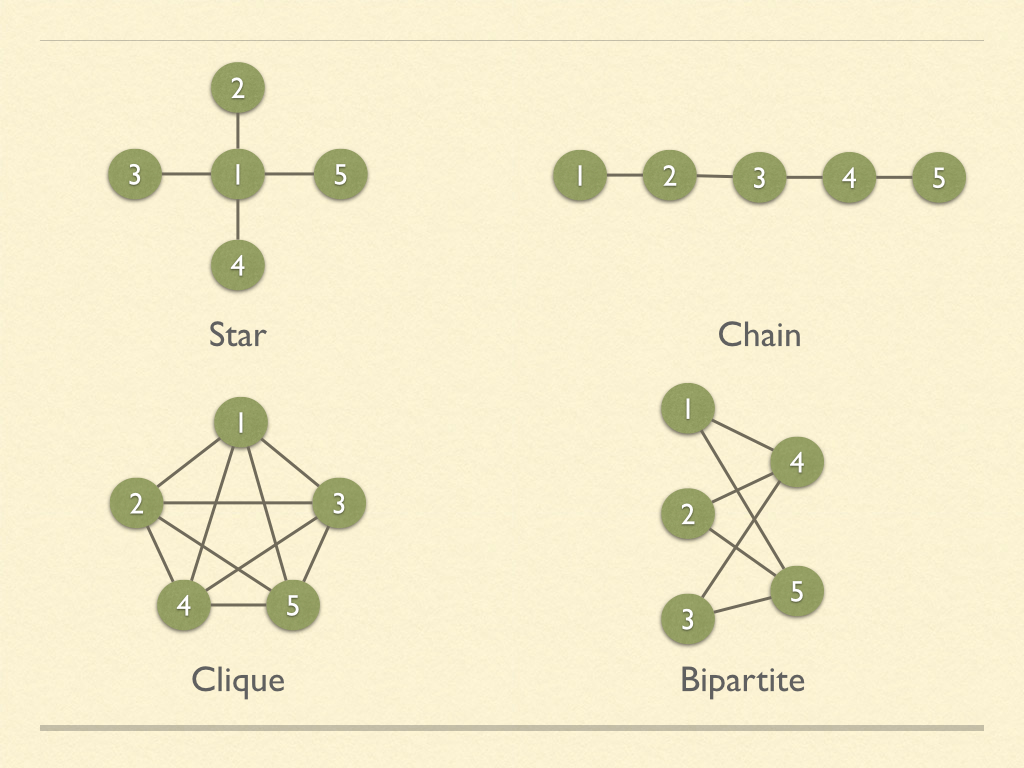
\includegraphics[width=0.6\textwidth]{FIG/testcase.jpg} \\
     %\psfig{figure=FIG/plot.ps,width=2in} \\
     % \psfig{figure=FIG/data.ps,width=2in} &
     % \psfig{figure=FIG/plot.ps,width=2in} \\
\end{tabular}
\caption{Test Case}
\label{fig:testcase}
\end{center}
\end{figure}

%%%%%%%%%%%%%%%%%%%%%%%%%%%%%%%%%%%%%%%%%%%%%%%%%%%%%%%%%%%

\subsection{Task 1: Degree Distribution}
\subsubsection{Accuracy Demonstration}
One way we use the veryify the result is to use the task case(which can be inferred manually). The reults we get from algorithm are as follows, which meet the values we expected.
\begin{verbatim}
Star:
 degree | count 
--------+-------
      1 |     4
      4 |     1

Chain:
 degree | count 
--------+-------
      1 |     2
      2 |     3

Clique:
 degree | count 
--------+-------
      4 |     5

Bipartite:
 degree | count 
--------+-------
      2 |     3
      3 |     2
\end{verbatim}

Another way is to check if the plot follows the power law in real dataset. We implemented the degree distribution method using SQL and performed the query on Facebook Social Circle dataset from SNAP
\footnote{SNAP: http://snap.stanford.edu/data/index.html}. The graph has 4039 vertices and 88234 edges. 

Figure \ref{fig:results} shows our results:
Figure \ref{fig:results}(a) gives a scatter-plot of the in-degree distribution on a log-log scale for the Facebook graph dataset.
Figure \ref{fig:results}(b) shows the out-degree distirbution.
X axis indicates the in-degree and y axis indicates the number of vertices which have the same in-degree or out-degree. 
According to the figures, We can easily observe the Power Law(heavy-tailed degree distribution) pattern.

\begin{figure}[htbf]
\begin{center}
\begin{tabular}{cc}
     % uncomment the next lines, and give the right ps files
     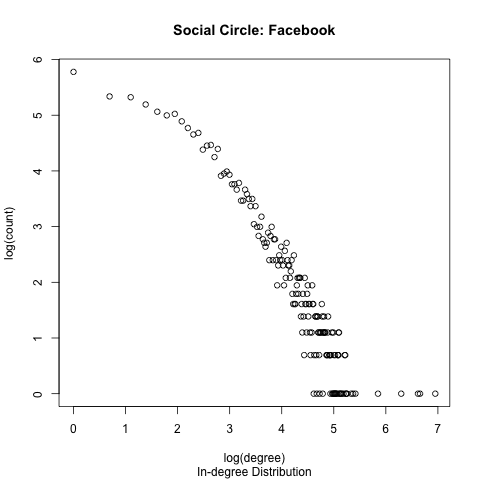
\includegraphics[width=0.5\textwidth]{FIG/in_degree.png} &
     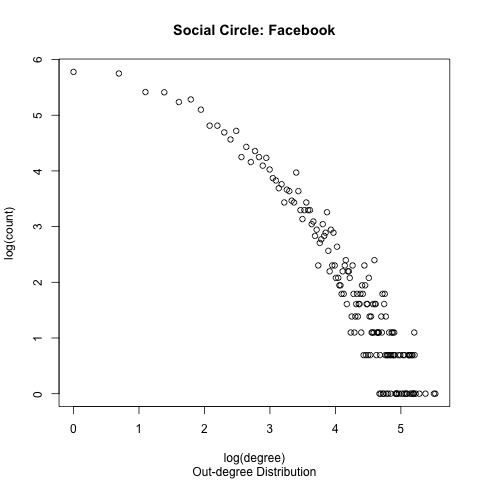
\includegraphics[width=0.5\textwidth]{FIG/out_degree.png} \\
     %\psfig{figure=FIG/plot.ps,width=2in} \\
     % \psfig{figure=FIG/data.ps,width=2in} &
     % \psfig{figure=FIG/plot.ps,width=2in} \\
    (a) & (b) 
\end{tabular}
\caption{The in-degree distribution plot(a) and out-degree distribution plot (b) on a log-log scale for Facebook graph dataset}
\label{fig:results}
\end{center}
\end{figure}

\subsubsection{Variety  Demonstration}
We perform the test on five 1M node datasets: web-Google(directed), social-Youtube, roadMap-PA, roadMap-CA, and roadMap-TX. Figure \ref{fig:results1} shows the result.\\
From the result we can find the heavy-tailed power law distribution from every figure, which shows that real dataset are very skewed distributed.\\
What we can also find is the difference between social network/web graph and road network graph. Road network turns out to have very small number in terms of degree. This actually make sense because degree represent the number of direct neighbours. While a webpage can link to hundreds of other webpages, or a person could have millions of follower on social network, a road in real life actually connect to only a few of roads.
\begin{figure}
    \centering
    \begin{subfigure}[htbp]{0.9\textwidth}
            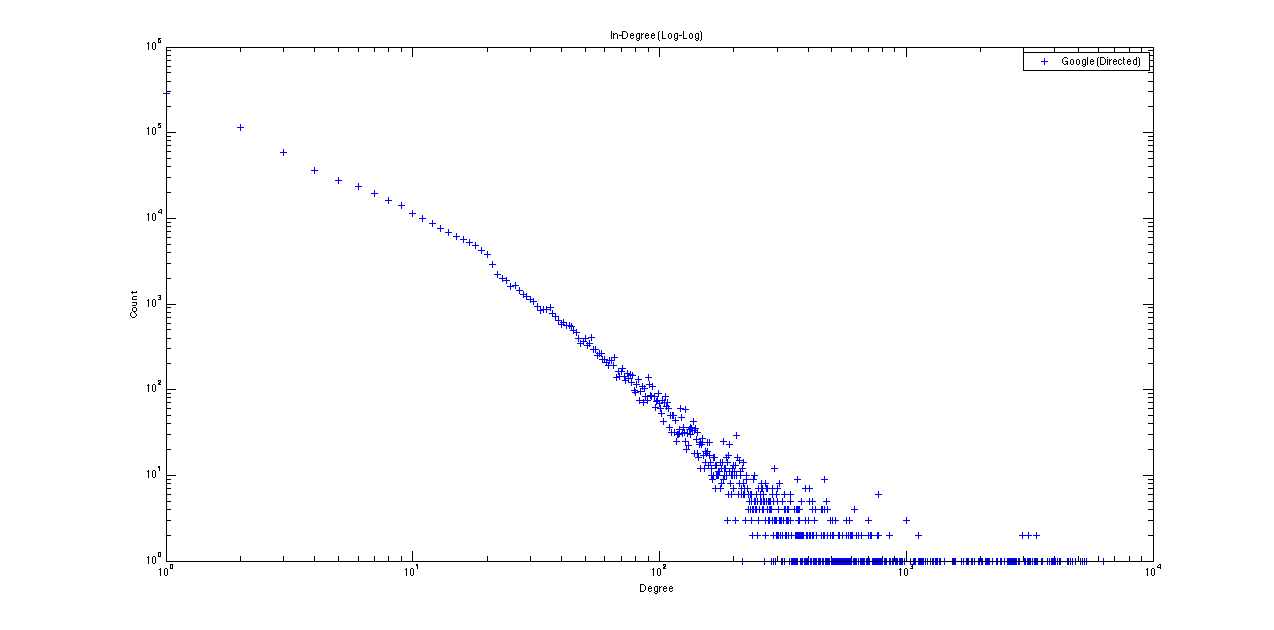
\includegraphics[width=\textwidth]{FIG/dd-google-in.png}
            \caption{Google in-Degree}
            \label{fig:dd-google-in}
    \end{subfigure}
    ~ %add desired spacing between images, e. g. ~, \quad, \qquad etc.
      %(or a blank line to force the subfigure onto a new line)
    \begin{subfigure}[htbp]{0.9\textwidth}
            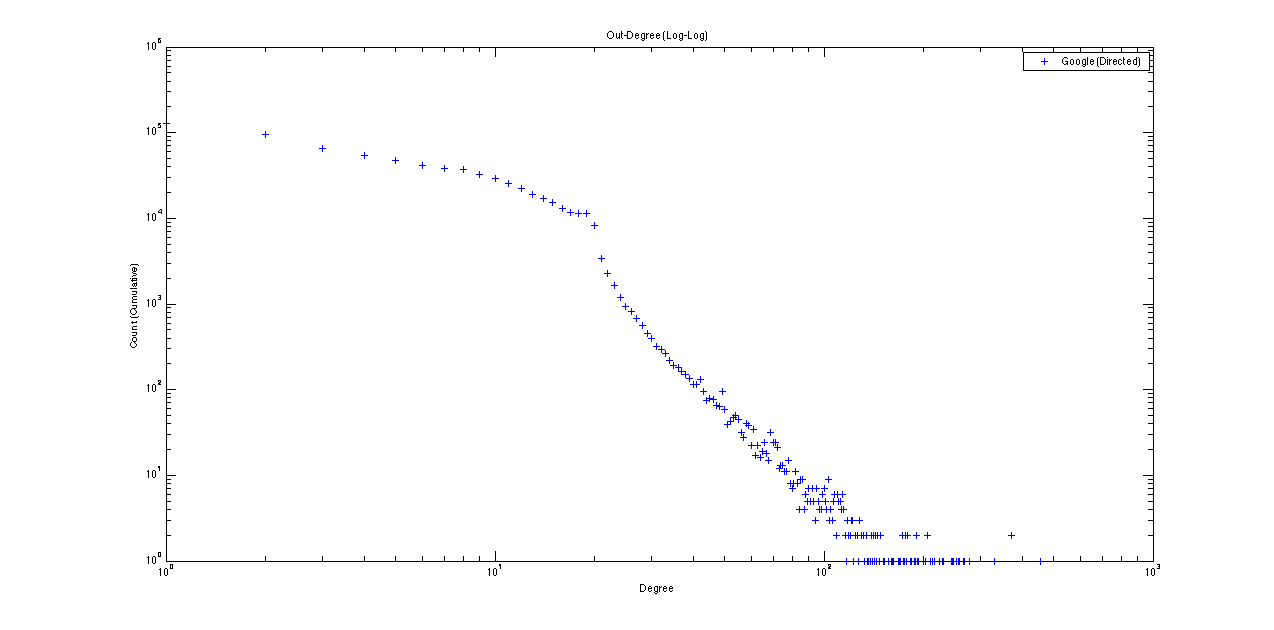
\includegraphics[width=\textwidth]{FIG/dd-google-out.png}
            \caption{Google out-Degree}
            \label{fig:dd-google-out}
    \end{subfigure}
    ~ %add desired spacing between images, e. g. ~, \quad, \qquad etc.
      %(or a blank line to force the subfigure onto a new line)
    \begin{subfigure}[htbp]{0.9\textwidth}
            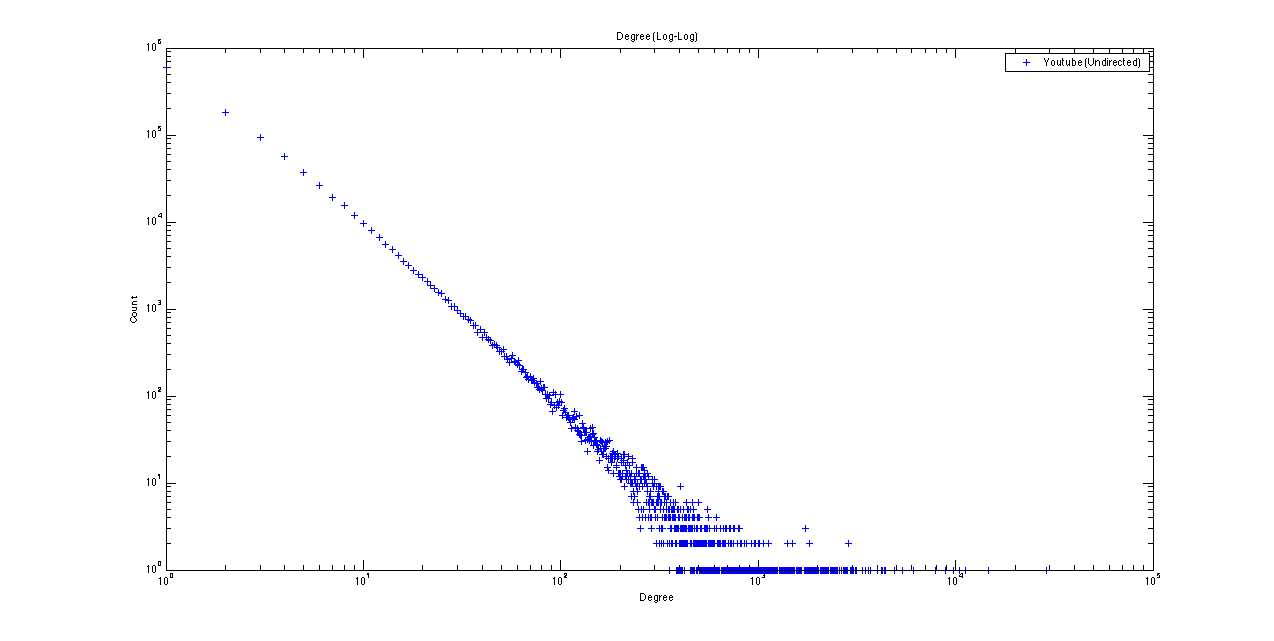
\includegraphics[width=\textwidth]{FIG/dd-youtube.png}
            \caption{Youtube}
            \label{fig:dd-youtube}
    \end{subfigure}
\end{figure} 

\addtocounter{figure}{-1}

\begin{figure} 
    \addtocounter{figure}{1}
    \centering 
        % ~ %add desired spacing between images, e. g. ~, \quad, \qquad etc.
          %(or a blank line to force the subfigure onto a new line)
        \begin{subfigure}[htbp]{0.9\textwidth}
                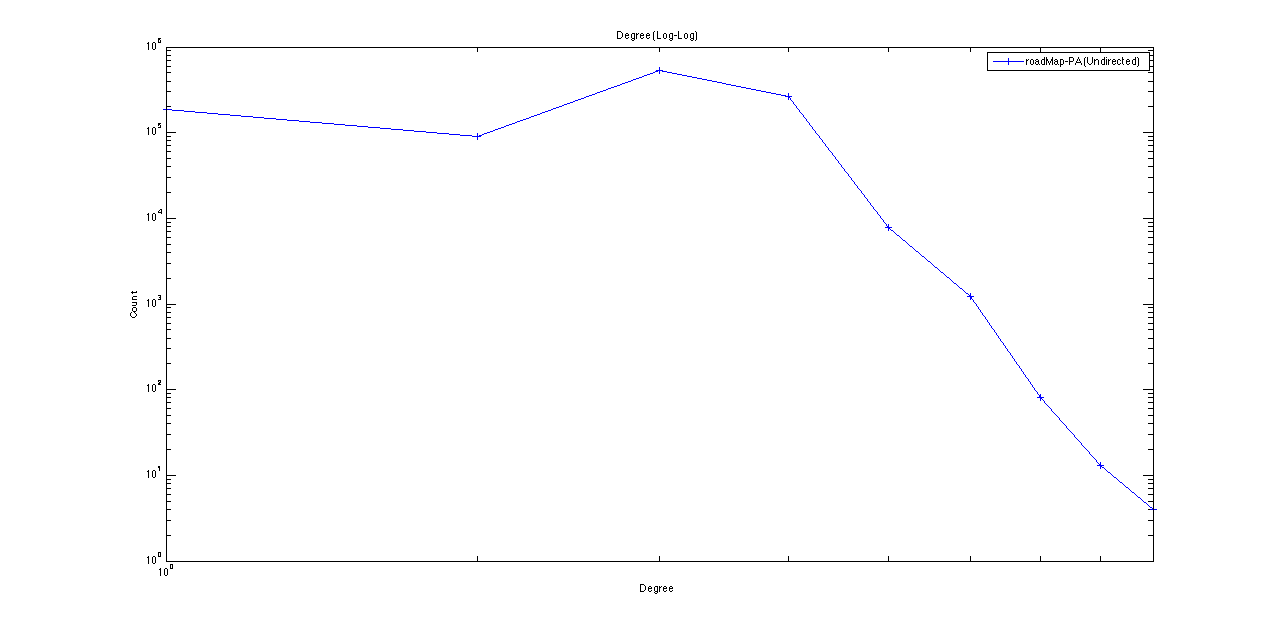
\includegraphics[width=\textwidth]{FIG/dd-pa.png}
                \caption{roadMap-PA}
                \label{fig:dd-pa}
        \end{subfigure}
        ~ %add desired spacing between images, e. g. ~, \quad, \qquad etc.
          %(or a blank line to force the subfigure onto a new line)
        \begin{subfigure}[htbp]{0.9\textwidth}
                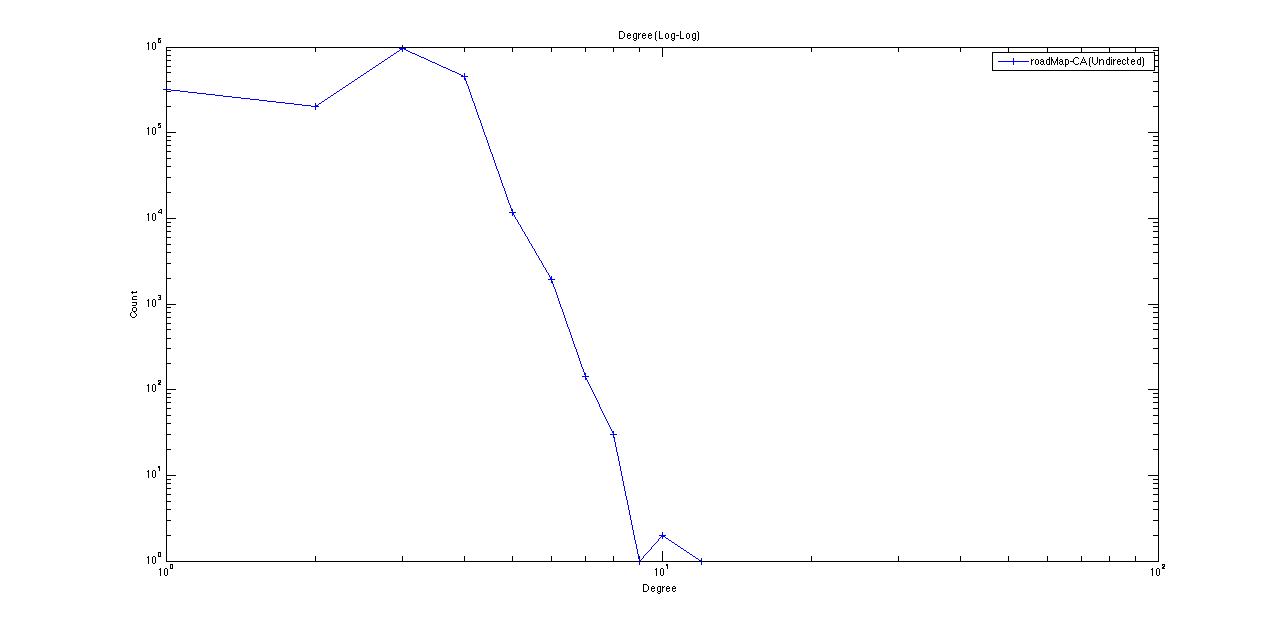
\includegraphics[width=\textwidth]{FIG/dd-ca.png}
                \caption{roadMap-CA}
                \label{fig:dd-ca}
        \end{subfigure}
        ~ %add desired spacing between images, e. g. ~, \quad, \qquad etc.
          %(or a blank line to force the subfigure onto a new line)
        \begin{subfigure}[htbp]{0.9\textwidth}
                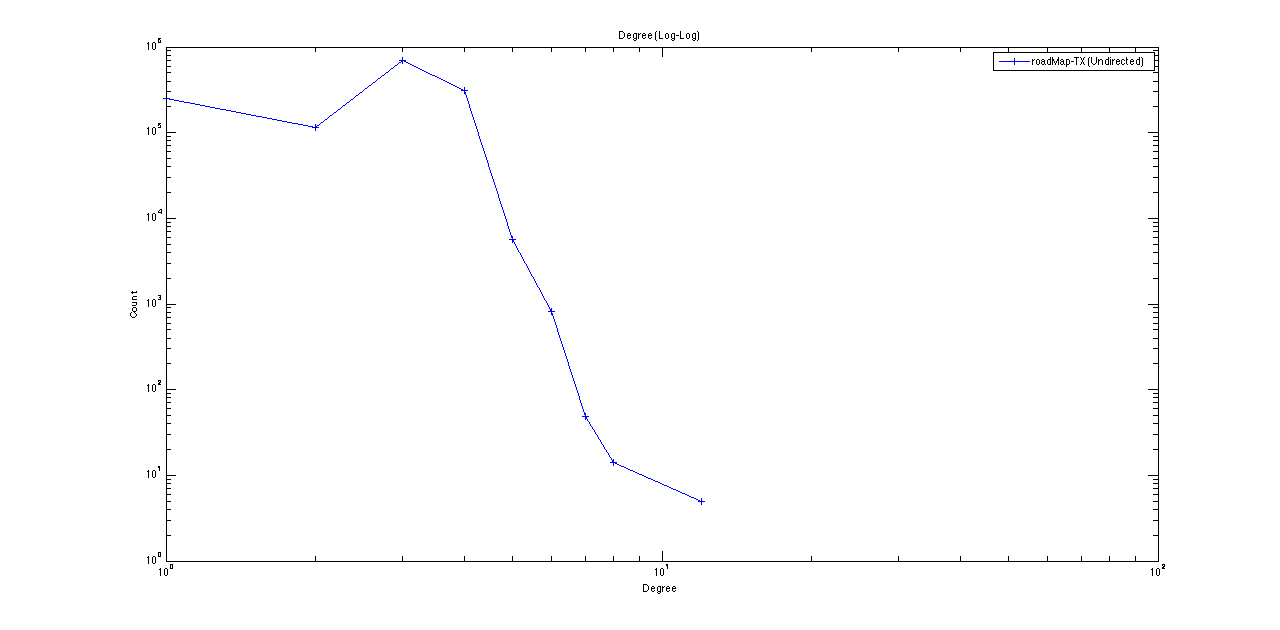
\includegraphics[width=\textwidth]{FIG/dd-tx.png}
                \caption{roadMap-TX}
                \label{fig:dd-tx}
        \end{subfigure}
        \caption{Degree Distribution}
        \label{fig:results1}
\end{figure}

%%%%%%%%%%%%%%%%%%%%%%%%%%%%%%%%%%%%%%%%%%%%%%%%%%%%%%%%%%%%%%%%%%%%%%%%%%%%%%%%%%%%%%%%%

\subsection{Task 2: Page Rank}
\subsubsection{Accuracy Demonstration}
We can also use the test case to tell if the PageRank computed by the algorithm is accurate. Consider the directed version of Star test case, where the hub(node 1) is pointed from every other nodes(node 2,3,4,5).\\
The result we get actually reflect the graph structure, where the hub has a higher rank and the rest of nodes share the same lower rank.
\begin{verbatim}
 v_row |       v_val        
-------+--------------------
     1 |                0.2
     2 | 0.0551136364533462
     3 | 0.0551136364533462
     4 | 0.0551136364533462
     5 | 0.0551136364533462
\end{verbatim}
Another thing we need to verify is the convergence of PageRank. Here we give the number of rank in iteration 10 and iteration 100. The result indicates that the rank computed by our algorithm coverges.
\begin{verbatim}
Iteration 10:
 v_row |       v_val        
-------+--------------------
     1 |                0.2
     2 | 0.0551136364533462
     3 | 0.0551136364533462
     4 | 0.0551136364533462
     5 | 0.0551136364533462
Iteration 100:
 v_row |       v_val        
-------+--------------------
     1 |                0.2
     2 | 0.0551136363636364
     3 | 0.0551136363636364
     4 | 0.0551136363636364
     5 | 0.0551136363636364
\end{verbatim}


\subsubsection{Variety Demonstration}
We perform the test on five 1M node datasets: web-Google(directed), social-Youtube, roadMap-PA, roadMap-CA, and roadMap-TX. Figure \ref{fig:results2} shows the result.\\
Notice that we are using cumulative count here in terms of the y-axis. That is, while x is the PageRank of a specific point, y is the number of points with greater PageRank value than that point.\\
From the figure we can figure out that both Youtube and Google graph follow the Power Law distribution of PageRank, which is pointed out in the paper \cite{Brin:1998:ALH:297810.297827}, while the roadMap datasets behave a little differently: only the latter part of the plot looks like power low distribution.

\begin{figure}
    \centering
    \begin{subfigure}[htbp]{0.9\textwidth}
            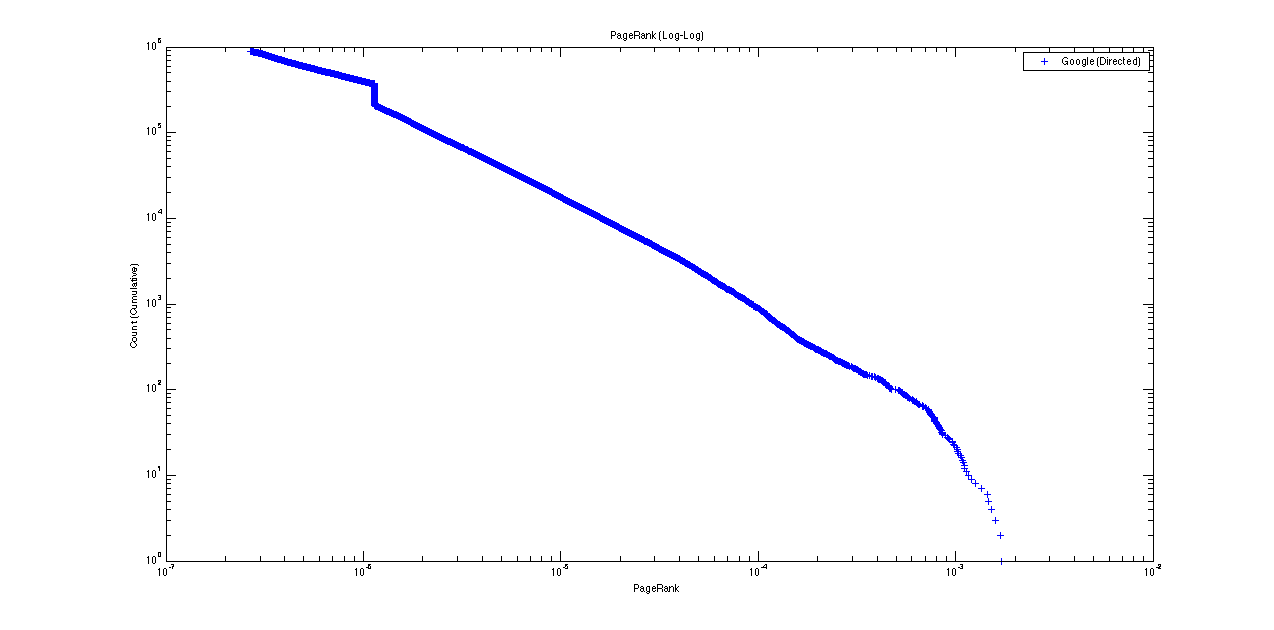
\includegraphics[width=\textwidth]{FIG/pr-google.png}
            \caption{Google}
            \label{fig:pr-google}
    \end{subfigure}
    ~ %add desired spacing between images, e. g. ~, \quad, \qquad etc.
      %(or a blank line to force the subfigure onto a new line)
    \begin{subfigure}[htbp]{0.9\textwidth}
            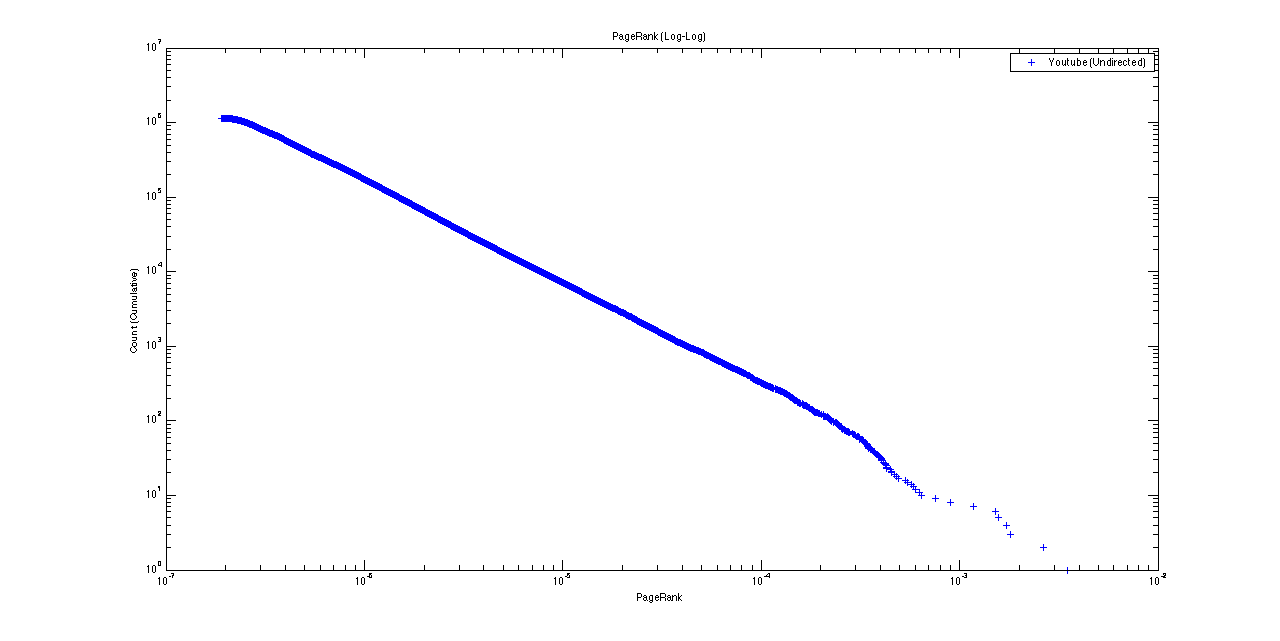
\includegraphics[width=\textwidth]{FIG/pr-youtube.png}
            \caption{Youtube}
            \label{fig:pr-youtube}
    \end{subfigure}
\end{figure} 

\addtocounter{figure}{-1}

\begin{figure} 
    \addtocounter{figure}{1}
    \centering 
        % ~ %add desired spacing between images, e. g. ~, \quad, \qquad etc.
          %(or a blank line to force the subfigure onto a new line)
        \begin{subfigure}[htbp]{0.9\textwidth}
                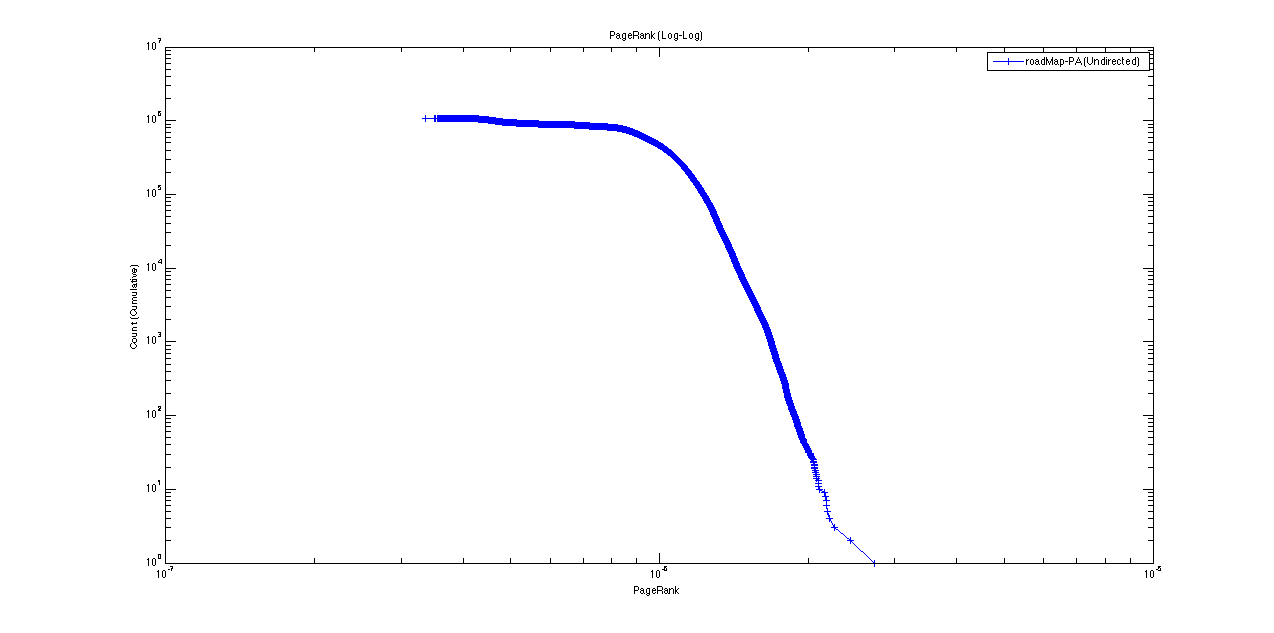
\includegraphics[width=\textwidth]{FIG/pr-pa.png}
                \caption{roadMap-PA}
                \label{fig:pr-pa}
        \end{subfigure}
        ~ %add desired spacing between images, e. g. ~, \quad, \qquad etc.
          %(or a blank line to force the subfigure onto a new line)
        \begin{subfigure}[htbp]{0.9\textwidth}
                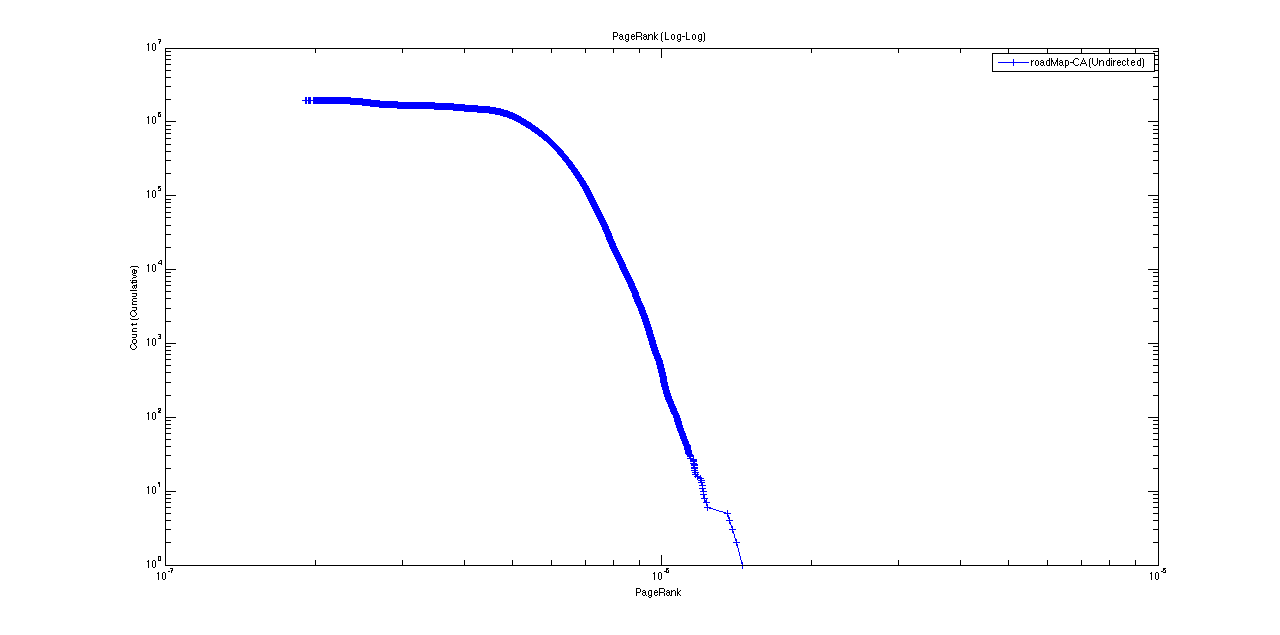
\includegraphics[width=\textwidth]{FIG/pr-ca.png}
                \caption{roadMap-CA}
                \label{fig:pr-ca}
        \end{subfigure}
        ~ %add desired spacing between images, e. g. ~, \quad, \qquad etc.
          %(or a blank line to force the subfigure onto a new line)
        \begin{subfigure}[htbp]{0.9\textwidth}
                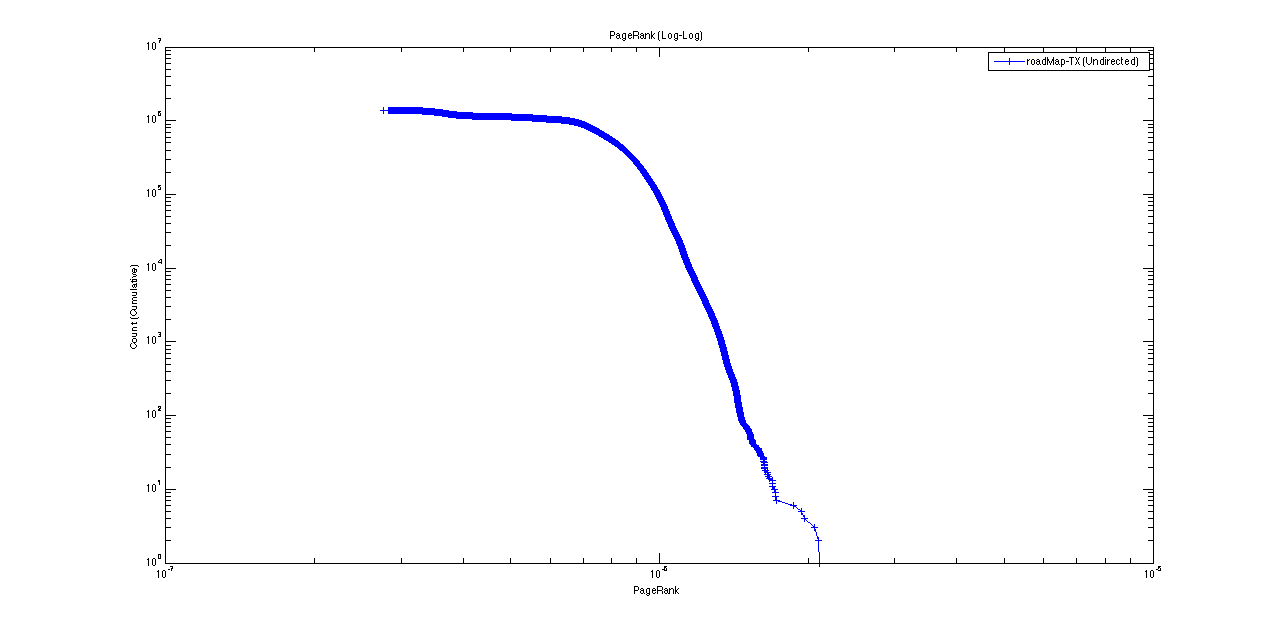
\includegraphics[width=\textwidth]{FIG/pr-tx.png}
                \caption{roadMap-TX}
                \label{fig:pr-tx}
        \end{subfigure}
        \caption{PageRank Distribution}
        \label{fig:results2}
\end{figure}

% We are in the progress of implementing Page Rank. We performed the first version of our code on Adjective-noun dataset from KONECT
% \footnote{KONECT: http://konect.uni-koblenz.de/networks/}. The graph has 86 vertices and 108 edges. 

% Figure \ref{fig:results2} shows our results. 
% X-axis indicates the number of nodes while y-axis gives the page rank.
% As can be seen in the graph, the nodes are normally distributed. Because this is a undirected graph, the page rank reveals the degree of each node.

% \begin{figure}[htbf]
% \begin{center}
% \begin{tabular}{cc}
%      % uncomment the next lines, and give the right ps files
%      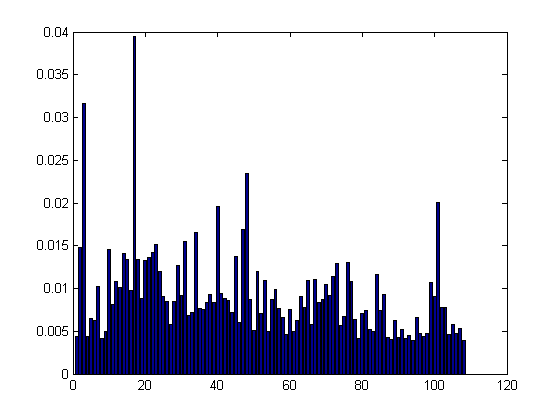
\includegraphics[width=0.6\textwidth]{FIG/task2.png} \\
%      %\psfig{figure=FIG/plot.ps,width=2in} \\
%      % \psfig{figure=FIG/data.ps,width=2in} &
%      % \psfig{figure=FIG/plot.ps,width=2in} \\
% \end{tabular}
% \caption{The Page-Rank plot for Adjective-noun dataset}
% \label{fig:results2}
% \end{center}
% \end{figure}

%%%%%%%%%%%%%%%%%%%%%%%%%%%%%%%%%%%%%%%%%%%%%%%%%%%%%%%%%%%%%%%%%%%%%%%%%%%%%%%%%%%%%%%%%

\subsection{Task 3: Connected Components}
\subsubsection{Accuracy Demonstration}
We use the test case to verify if the connected components computed by the algorithm is accurate. \\
Here we combines 4 test cases into one graph: node 1-5 belongs to Star graph; node 11-15 belongs to chain graph; node 21-25 belongs to clique graph; node 31-35 belongs to bipartite.\\
As for result, we expect to see four component each with size of 5. And the result are given as follows, which satisfies our expectation.\\
\begin{verbatim}
 node | comp 
------+------
    1 |    1
    2 |    1
    3 |    1
    4 |    1
    5 |    1
   11 |   11
   12 |   11
   13 |   11
   14 |   11
   15 |   11
   21 |   21
   22 |   21
   23 |   21
   24 |   21
   25 |   21
   31 |   31
   32 |   31
   33 |   31
   34 |   31
   35 |   31
\end{verbatim}
As for the convergence test, we modify the test case above by connecting four sub graph together, i.e. add three edges: 1-11, 11-21, 21-31. From the result given, we can tell that it costs five round for the algorithm to converge and the whole graph is formed in to a giant connected component, which is exactly what we expect.

\begin{verbatim}
 node | comp 
------+------
    1 |    1
    2 |    1
    3 |    1
    4 |    1
    5 |    1
   11 |    1
   12 |    1
   13 |    1
   14 |    1
   15 |    1
   21 |    1
   22 |    1
   23 |    1
   24 |    1
   25 |    1
   31 |    1
   32 |    1
   33 |    1
   34 |    1
   35 |    1
(20 rows)

Time: 0.813 ms
 round | gcc_count 
-------+-----------
     1 |         6
     2 |         8
     3 |        14
     4 |        17
     5 |        20
\end{verbatim}

\subsubsection{Variety Demonstration}
We perform the test on five 1M node datasets: web-Google(directed), social-Youtube, roadMap-PA, roadMap-CA, and roadMap-TX. Figure \ref{fig:results3} shows the result of convergence.\\
From the figure, we can see that Google and Youtube graph converge in around 10 iterations. However, roadMap-PA graph did not reach to convergen after the maximum iteration(which is set to 256). \\
The big difference from social network/web graph and roadnet graph still exists here. Although it takes only a few iteration for the network/graph to converge, the road graphs take far more rounds. The situation makes good sense because it exactly reflect the effect of small diameter/small world/six degree of seperation in terms of social network and web graph. \\
Meanwhile, the common sense confirms us that road networks are supposed to have long chain and large radius/diameter, which means far more iterations for the connected components to converge.\\
\begin{figure}
    \centering
    \begin{subfigure}[htbp]{0.8\textwidth}
            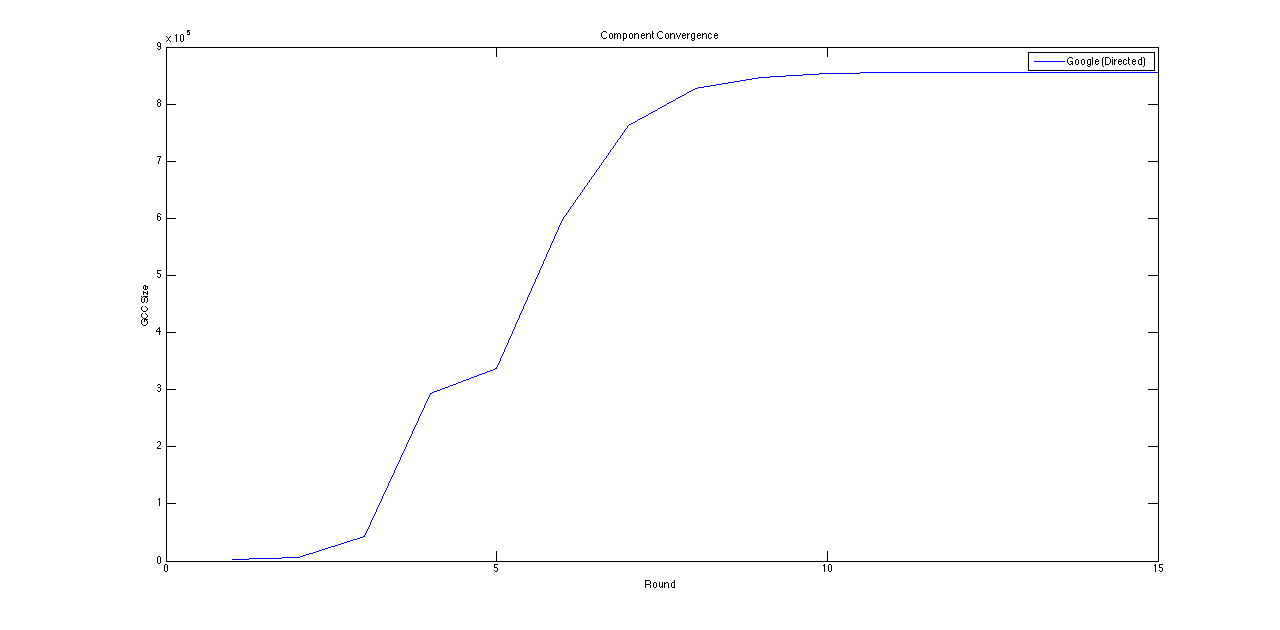
\includegraphics[width=\textwidth]{FIG/cp-google-c.png}
            \caption{Google}
            \label{fig:cp-google-c}
    \end{subfigure}
    ~ %add desired spacing between images, e. g. ~, \quad, \qquad etc.
      %(or a blank line to force the subfigure onto a new line)
    \begin{subfigure}[htbp]{0.8\textwidth}
            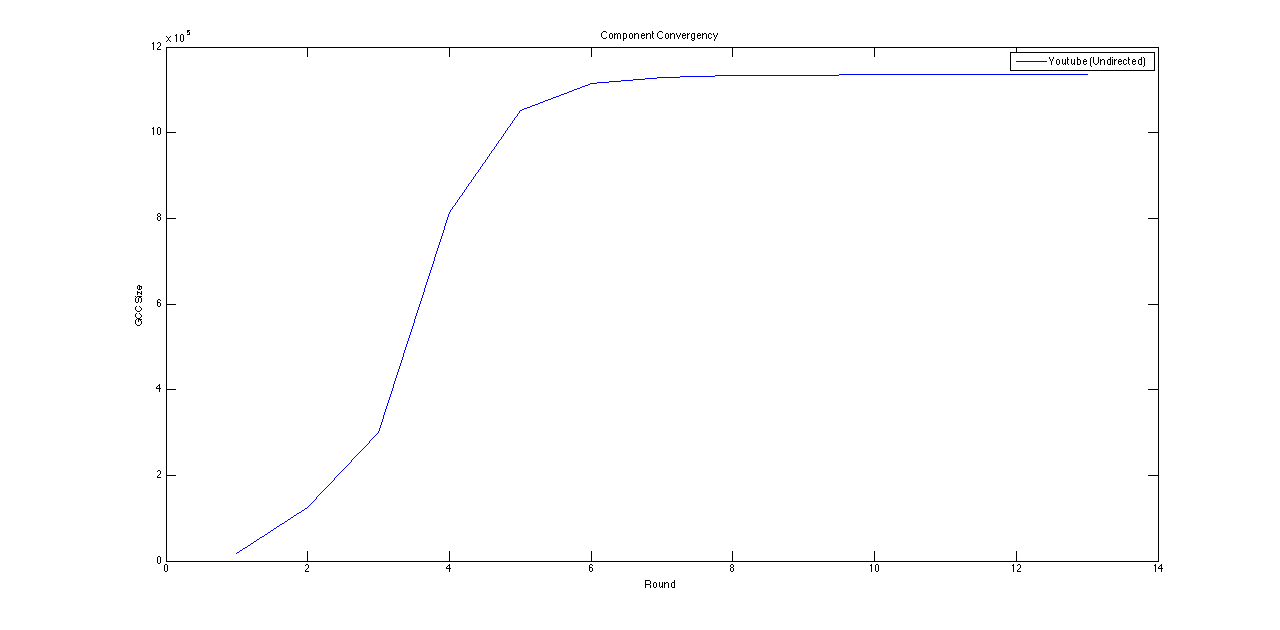
\includegraphics[width=\textwidth]{FIG/cp-youtube-c.png}
            \caption{Youtube}
            \label{fig:cp-youtube-c}
    \end{subfigure}
    ~ %add desired spacing between images, e. g. ~, \quad, \qquad etc.
      %(or a blank line to force the subfigure onto a new line)
    \begin{subfigure}[htbp]{0.8\textwidth}
            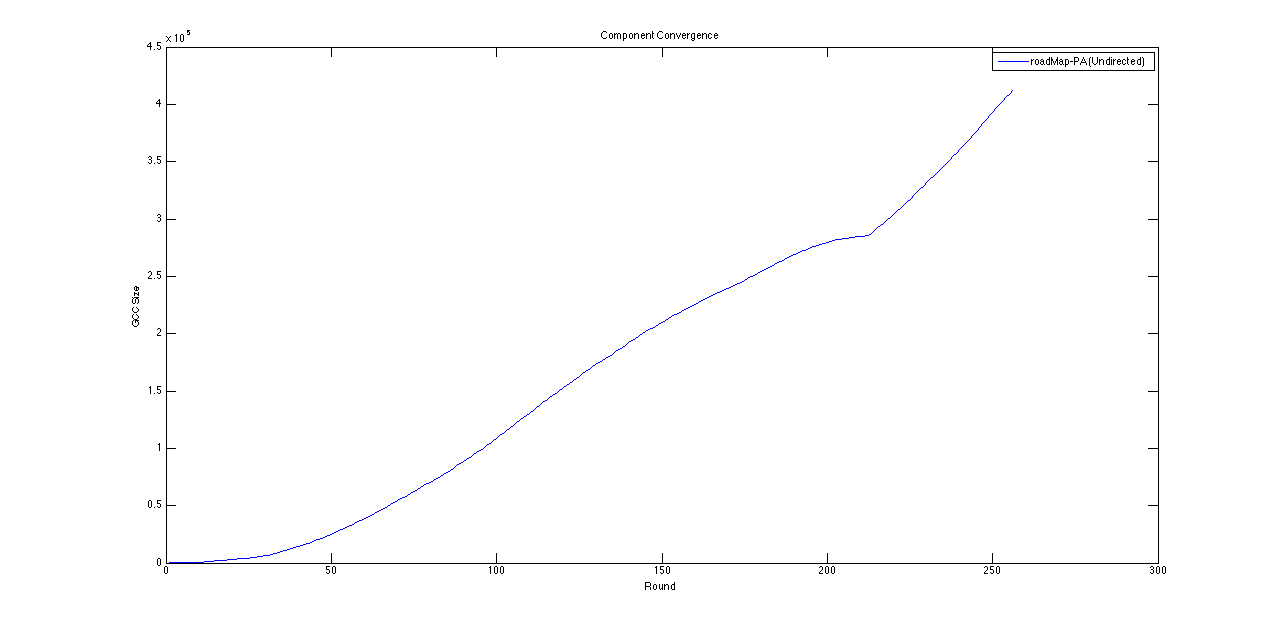
\includegraphics[width=\textwidth]{FIG/cp-pa-c.png}
            \caption{}
            \label{fig:cp-pa-c.png}
    \end{subfigure}
    \caption{Component Convergence}
        \label{fig:results3}
\end{figure} 

We also give the plot of connected component distribution. Notice that Youtube graph is actually all-connected and there is only one GCC. Therefore, we only give the plot of Google, roadMap-PA after 20 iterations, roadMap-PA after 256 iterations(which took over 22000000 ms to run), roadMap-CA after 10 iterations and roadMap-TX after 10 iterations.\\
Figure \ref{fig:results3-1} shows the result of component plot.
\begin{figure}
    \centering
    \begin{subfigure}[htbp]{0.8\textwidth}
            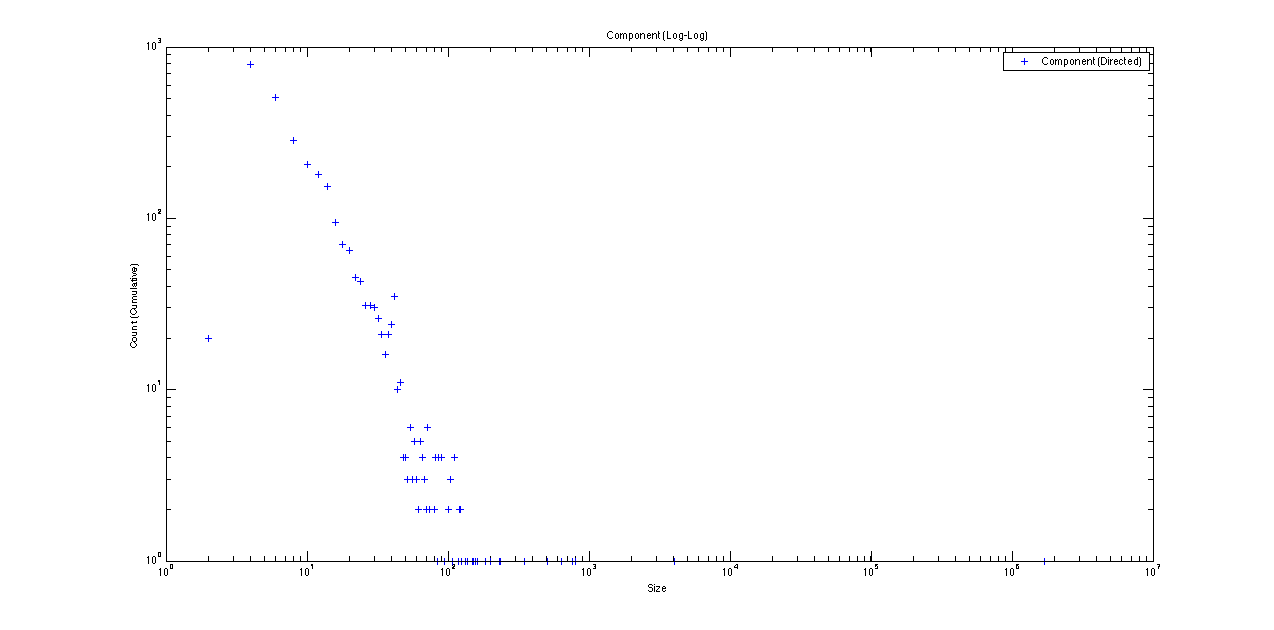
\includegraphics[width=\textwidth]{FIG/cp-google.png}
            \caption{Google}
            \label{fig:cp-google}
    \end{subfigure}
    ~ %add desired spacing between images, e. g. ~, \quad, \qquad etc.
      %(or a blank line to force the subfigure onto a new line)
    \begin{subfigure}[htbp]{0.8\textwidth}
            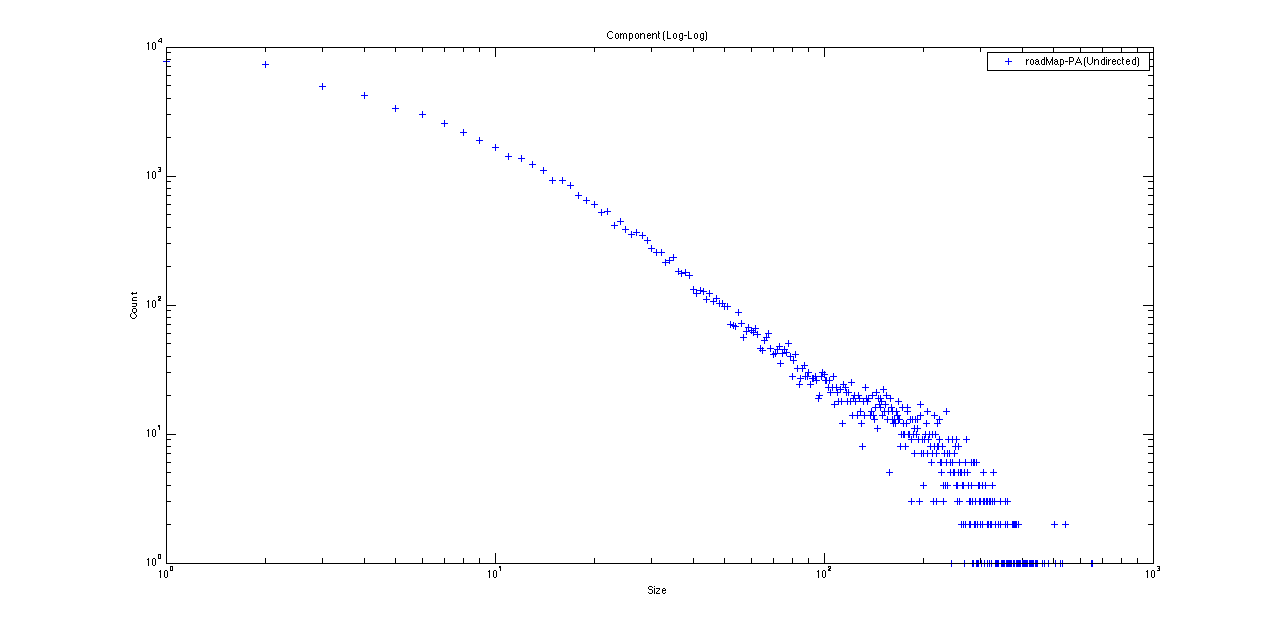
\includegraphics[width=\textwidth]{FIG/cp-pa-20.png}
            \caption{roadMap-PA 20 iterations}
            \label{fig:cp-pa-20}
    \end{subfigure}
    ~ %add desired spacing between images, e. g. ~, \quad, \qquad etc.
      %(or a blank line to force the subfigure onto a new line)
    \begin{subfigure}[htbp]{0.8\textwidth}
            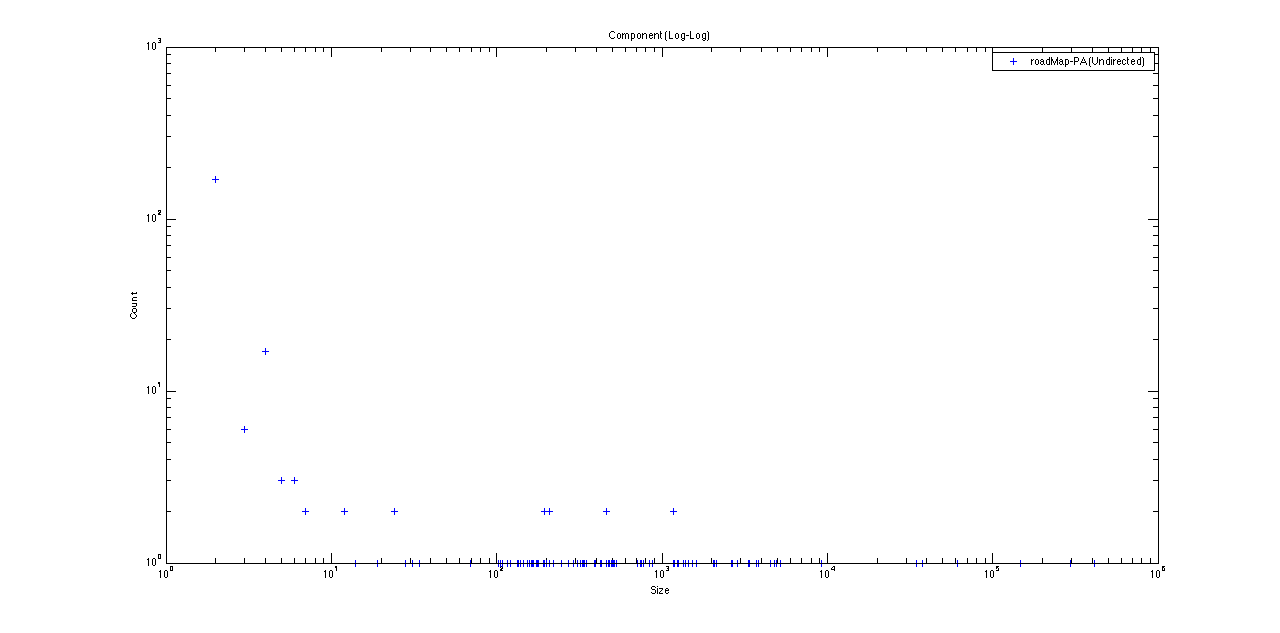
\includegraphics[width=\textwidth]{FIG/cp-pa.png}
            \caption{roadMap-PA 256 iterations}
            \label{fig:cp-pa.png}
    \end{subfigure}
\end{figure}

\addtocounter{figure}{-1}

\begin{figure} 
    \addtocounter{figure}{1}
    \centering 
        % ~ %add desired spacing between images, e. g. ~, \quad, \qquad etc.
          %(or a blank line to force the subfigure onto a new line)
        \begin{subfigure}[htbp]{0.8\textwidth}
                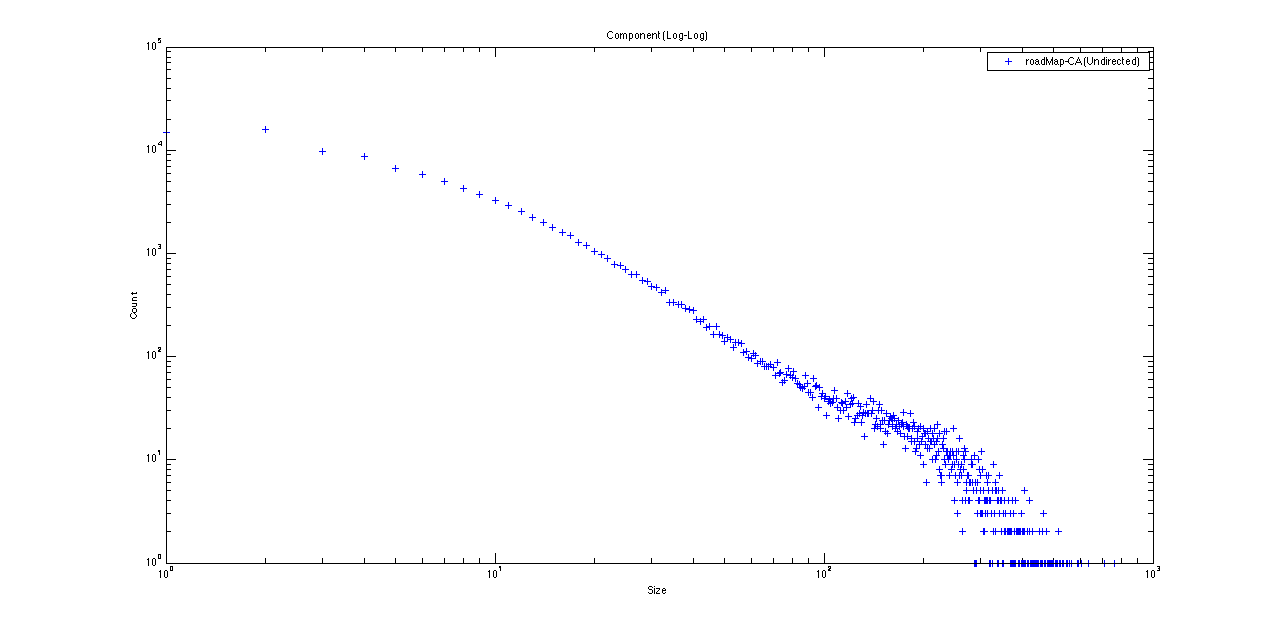
\includegraphics[width=\textwidth]{FIG/cp-ca.png}
                \caption{roadMap-CA 10 iterations}
                \label{fig:cp-pa}
        \end{subfigure}
        ~ %add desired spacing between images, e. g. ~, \quad, \qquad etc.
          %(or a blank line to force the subfigure onto a new line)
        \begin{subfigure}[htbp]{0.8\textwidth}
                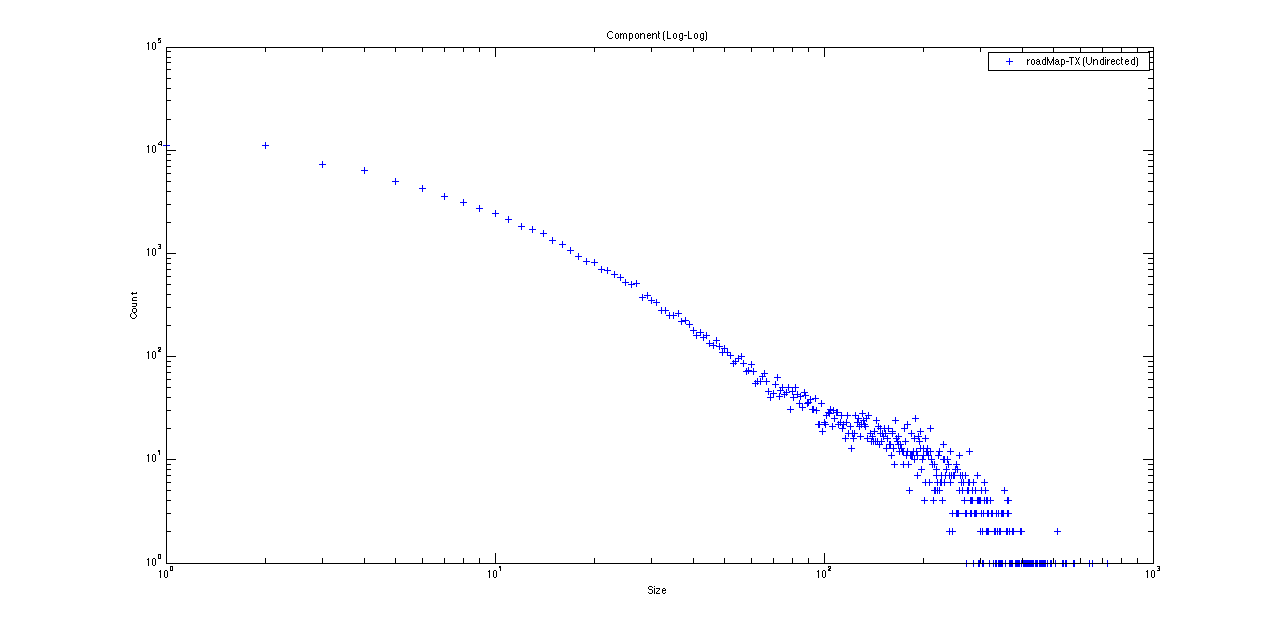
\includegraphics[width=\textwidth]{FIG/cp-tx.png}
                \caption{roadMap-TX 10 iterations}
                \label{fig:cp-tx}
        \end{subfigure}
    \caption{Component Distribution}
    \label{fig:results3-1}
\end{figure} 

%%%%%%%%%%%%%%%%%%%%%%%%%%%%%%%%%%%%%%%%%%%%%%%%%%%%%%%%%%%%%%%%%%%%%%%%%%%%%%%%

\subsection{Task 4: Radius}
\subsubsection{Accuracy Demonstration}
We examine a small test case on a undirected graph with 8 nodes. Figure \ref{fig:results4} shows the graph structire. \\
It is obvious to tell from the image that Node 1 and Node 5 have the largest radium 5, which is the diameter of this graph. \\
Running the algrithm on the graph, we get the output as follows, which is in line with the result from the image.
\begin{verbatim}
postgres=# select * from radius(20);
 node | radius 
------+--------
    1 |      5
    2 |      4
    3 |      3
    4 |      4
    5 |      5
    6 |      2
    7 |      2
    8 |      2
(8 rows)
\end{verbatim}

\begin{figure}[htbf]
\begin{center}
\begin{tabular}{cc}
     % uncomment the next lines, and give the right ps files
     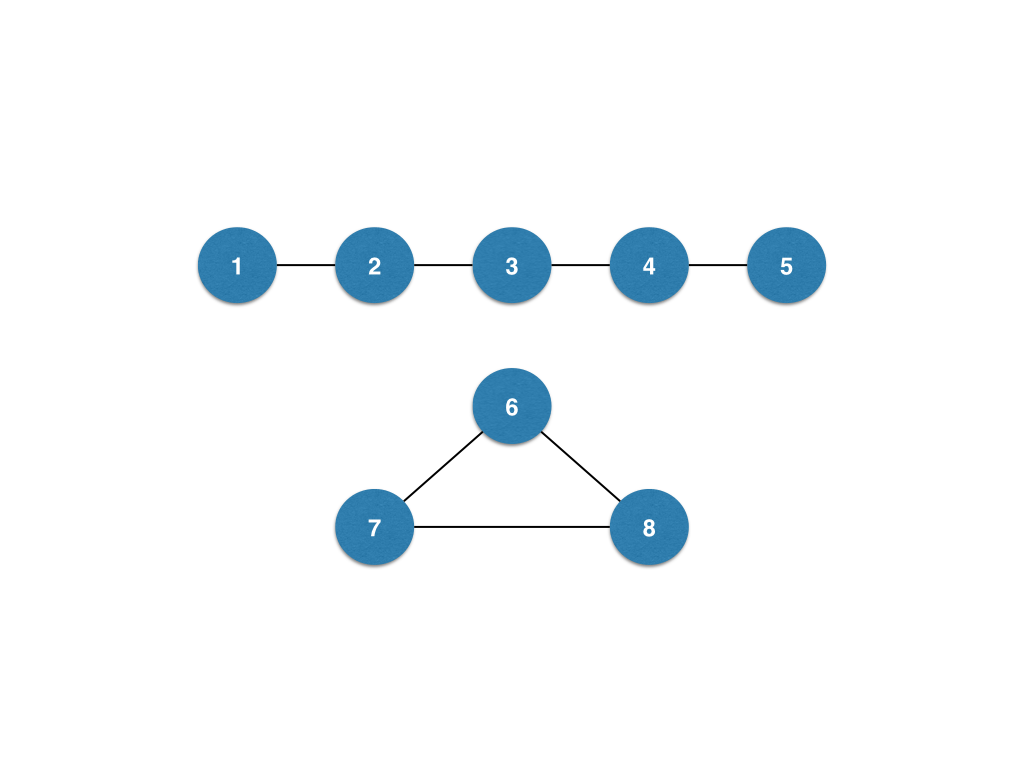
\includegraphics[width=0.6\textwidth]{FIG/task4.png} \\
     %\psfig{figure=FIG/plot.ps,width=2in} \\
     % \psfig{figure=FIG/data.ps,width=2in} &
     % \psfig{figure=FIG/plot.ps,width=2in} \\
\end{tabular}
\caption{Test case graph for Radium and Diameter}
\label{fig:results4}
\end{center}
\end{figure}

\subsubsection{Variety Demonstration}
We perform the test on two 1M node datasets: web-Google(directed) and Youtube. Figure \ref{fig:results3-1} shows the result. \\
Since the iteration stop earlier than maximum iteration(256), we guarantee that radius are converge here. \\
As we mentioned in the last section that real world graphs like road network tend to have chains and large radius, we skip the test here considering its running time.

\begin{figure}
    \centering
    \begin{subfigure}[htbp]{0.8\textwidth}
            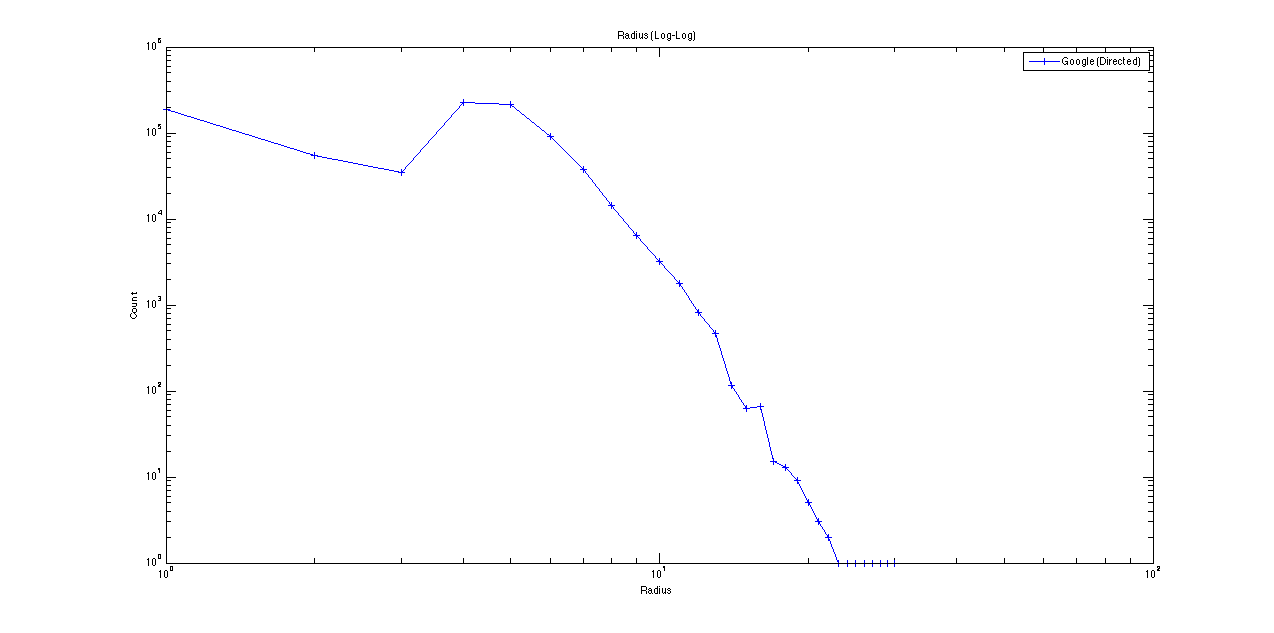
\includegraphics[width=\textwidth]{FIG/rd-google.png}
            \caption{Google}
            \label{fig:rd-google}
    \end{subfigure}
    ~ %add desired spacing between images, e. g. ~, \quad, \qquad etc.
      %(or a blank line to force the subfigure onto a new line)
    \begin{subfigure}[htbp]{0.8\textwidth}
            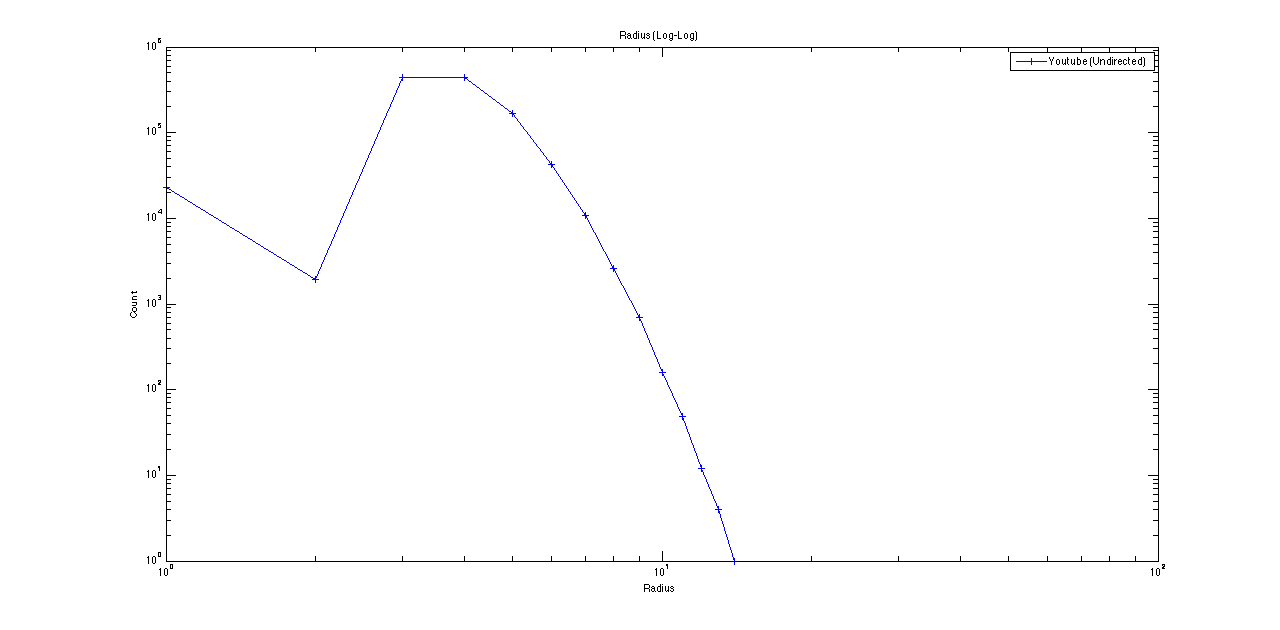
\includegraphics[width=\textwidth]{FIG/rd-youtube.png}
            \caption{Youtube}
            \label{fig:rd-youtube}
    \end{subfigure}
    \caption{Radius Distribution}
        \label{fig:results3-1}
\end{figure}

%%%%%%%%%%%%%%%%%%%%%%%%%%%%%%%%%%%%%%%%%%%%%%%%%%%%%%%%%%%%%%%%%%%%%%%%%%%%%%%%%%%%%%%%%%%%%

\subsection{Task 5: Eigenvalues}
{Accuracy Demonstration}
First, we successfully implemented Lanczos-NO algorithm. But we found there were some eigenvalues missing. We thought it was because the rounding errors from floating-point calculations as its said in the paper. But after we implemented Lanczos-SO algorithm, there are still eigenvalues missing. \\
In the following test, we found out that the correctness of calculating eigenvalues by Lanczos is largely related by the number of iteration and the initial value chosen. The more the number of iteration, the more correctness brought to eigenvalue calculation, but the also the more calculation time it takes. \\
As a treat off, we only calculate the first 10 eigenvalues in the following experiments, as shown in Figure \ref{fig:results5-1}.\\
\begin{figure}[htbf]
\begin{center}
\begin{tabular}{cc}
     % uncomment the next lines, and give the right ps files
     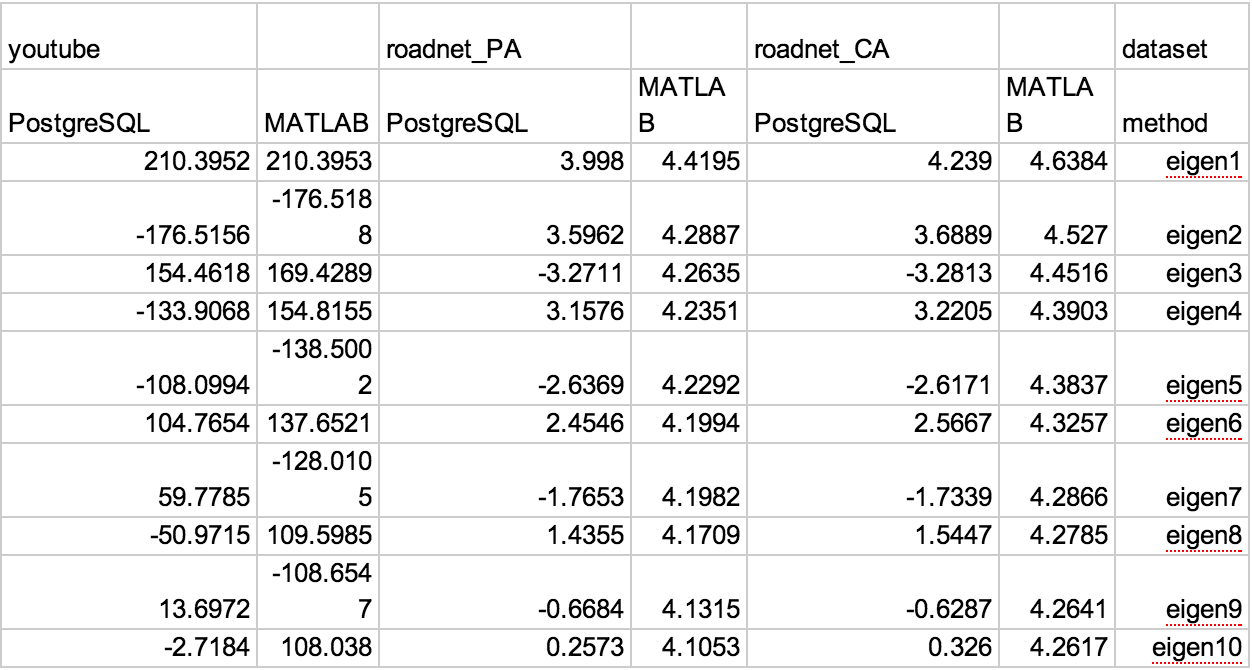
\includegraphics[width=0.8\textwidth]{FIG/tab.png} \\
     %\psfig{figure=FIG/plot.ps,width=2in} \\
     % \psfig{figure=FIG/data.ps,width=2in} &
     % \psfig{figure=FIG/plot.ps,width=2in} \\
\end{tabular}
\caption{Eigenvalues and rank plot}
\label{fig:results5-1}
\end{center}
\end{figure}
As can be seen from the eigenvalues calculated by us and the ones calculated by MATLAB. Only the first few result are corresponding to the greatest eigenvalue that calculated by MATLAB. \\
Our conclusion is that Lanczos algorithm with small number of iteration K, is not suitable to calculate the greatest K eigenvalues of a matrix, because it may not find them all, like the “youtube” dataset. And the calculation result is extremely bad when eigenvalues are close to each other, like “roadnet” datasets. \\
Despite of this, we found out some pattern of the eigenvalues calculated by the Lanczos algorithm. Take a simple dataset - “adjnoun” - as example. The eigenvalue-rank plot is as follows in Figure \ref{fig:results5}. \\
As can be seen in the graph, the first few eigenvalues are alternately greater or smaller than 0, and the absolute value of eigenvalues are getting smaller.

\begin{figure}[htbf]
\begin{center}
\begin{tabular}{cc}
     % uncomment the next lines, and give the right ps files
     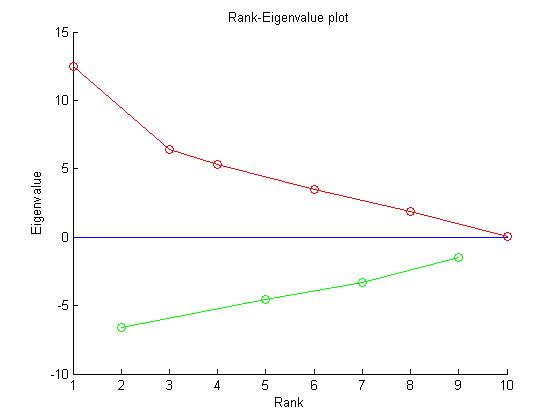
\includegraphics[width=0.8\textwidth]{FIG/task5.jpg} \\
     %\psfig{figure=FIG/plot.ps,width=2in} \\
     % \psfig{figure=FIG/data.ps,width=2in} &
     % \psfig{figure=FIG/plot.ps,width=2in} \\
\end{tabular}
\caption{Eigenvalues-rank plot for adjnoun dataset}
\label{fig:results5}
\end{center}
\end{figure}

\subsubsection{Varienty Demonstration}
We perform the test on several 1M nodes datasets: social-Youtube, roadMap-PA and roadMap-CA. Figure \ref{fig:results5-2} shows the result.\\
\begin{figure}
    \centering
    \begin{subfigure}[htbp]{0.6\textwidth}
            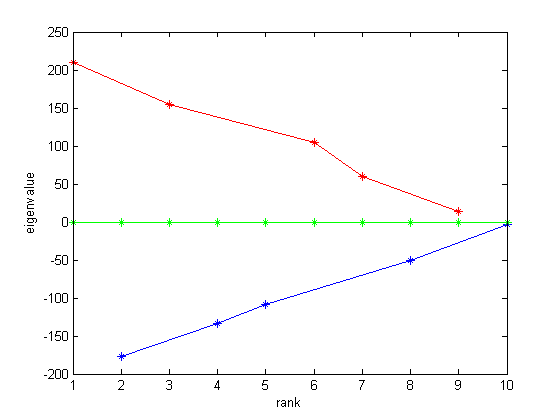
\includegraphics[width=\textwidth]{FIG/ei-youtube.png}
            \caption{Youtube}
            \label{fig:ei-youtube}
    \end{subfigure}
    ~ %add desired spacing between images, e. g. ~, \quad, \qquad etc.
      %(or a blank line to force the subfigure onto a new line)
    \begin{subfigure}[htbp]{0.6\textwidth}
            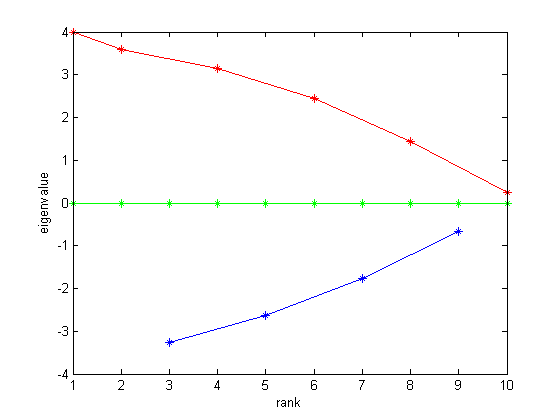
\includegraphics[width=\textwidth]{FIG/ei-pa.png}
            \caption{roadMap-PA}
            \label{fig:ei-pa}
    \end{subfigure}
    ~ %add desired spacing between images, e. g. ~, \quad, \qquad etc.
      %(or a blank line to force the subfigure onto a new line)
    \begin{subfigure}[htbp]{0.6\textwidth}
            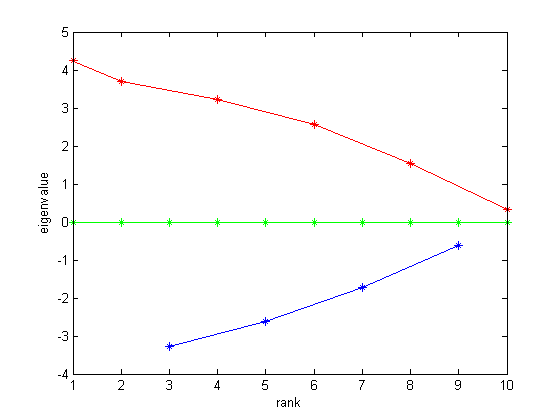
\includegraphics[width=\textwidth]{FIG/ei-ca.png}
            \caption{roadMap-CA}
            \label{fig:ei-ca.png}
    \end{subfigure}
    \caption{Eigenvalues and rank plot}
        \label{fig:results5-2}
\end{figure} 

%%%%%%%%%%%%%%%%%%%%%%%%%%%%%%%%%%%%%%%%%%%%%%%%%%%%%%%%%%%%%%%%%%%%%%%%%%%%%%%%%%

\subsection{Task 6: Belief Propagation}
\subsubsection{Accuracy Demonstration}
First, We want to check if the algorithm is able to give the correct inference of unlabed node. \\
We examine a small test case on a undirected graph with 4 nodes. Figure \ref{fig:results6} shows the graph structure. Given the label and initial belief of node 1, 2, 3, we intend to infer the label of node 4. \\
As for the intial belief, we set node 1=0.4(label: +), node 2=-0.4(label: -), node 3=0.3(label: +), and we leave node 4 = 0(lable: unknown). From the architecture of the graph, we can easily reach the conclusion that node 4 is more likely to be labeled as +(i.e. belief(node 4) > 0).\\
After performing the FastBP algorithm on the test graph, we have the output as follows. The node 4 is classified as +, which is what we expect.

\begin{verbatim}
postgres=# SELECT * from bp(20);
 v_row |       v_val        
-------+--------------------
     1 |  0.273209372007041
     2 | -0.198949408545921
     3 |  0.159512788522935
     4 | 0.0141145717811318
(4 rows)
\end{verbatim}

One thing worths noticing is that as $h_h$ serve as “about-half” homophily factor according to FastBP paper\cite{koutra2011unifying}. $h_h$ close to -0.5 means strong heterophily, while $h_h$ close to 0.5 means strong homophily. Therefore, we can also heterophily inference on the graph by setting $h_h$ to be negative.\\
Second, we want to check if the algorithm can converge. We compare the result after 10 iterations, 50 iterations and 100 iterations, which shows that the FastBP algorithm does converge.

\begin{verbatim}
10 iterations:
 v_row |         v_val         
-------+-----------------------
     1 |     0.288775545358658
     2 |    -0.264187325537205
     3 |     0.222905980050564
     4 | -0.000686401128768922

50 iterations:
 v_row |       v_val        
-------+--------------------
     1 |  0.273209372007041
     2 | -0.198949408545921
     3 |  0.159512788522935
     4 | 0.0141145717811318

100 iterations:
 v_row |       v_val        
-------+--------------------
     1 |  0.272932111246243
     2 | -0.197774913230647
     3 |  0.158338293512337
     4 | 0.0143918324157287
\end{verbatim}

\begin{figure}[htbf]
\begin{center}
\begin{tabular}{cc}
     % uncomment the next lines, and give the right ps files
     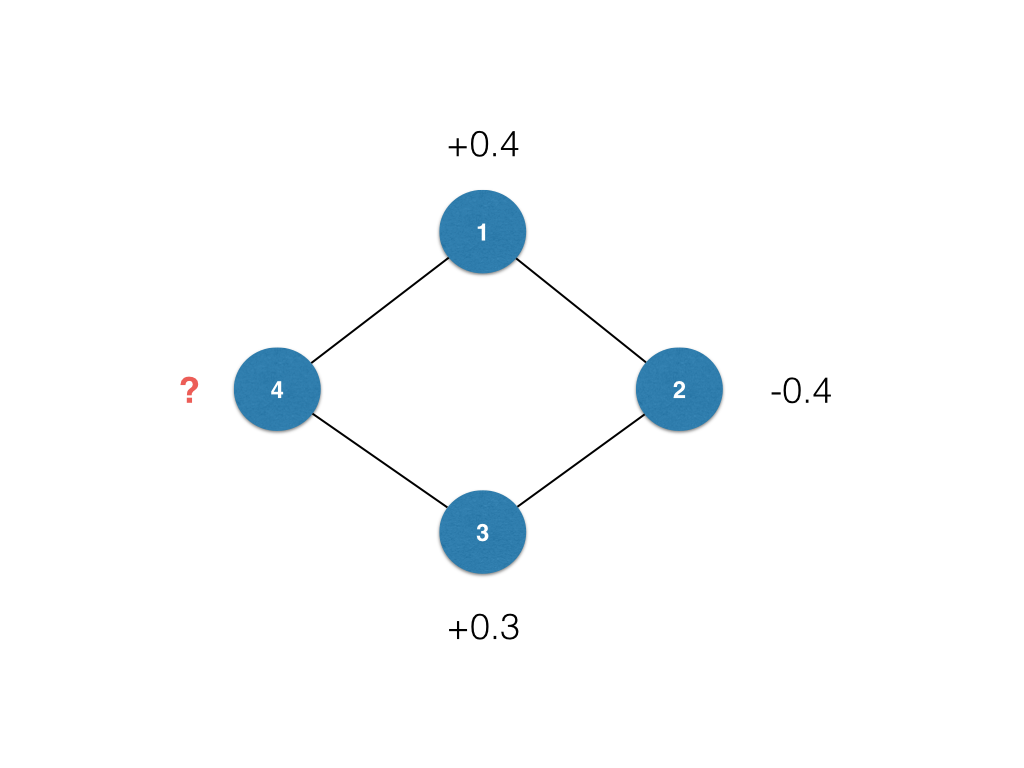
\includegraphics[width=0.6\textwidth]{FIG/task6.png} \\
     %\psfig{figure=FIG/plot.ps,width=2in} \\
     % \psfig{figure=FIG/data.ps,width=2in} &
     % \psfig{figure=FIG/plot.ps,width=2in} \\
\end{tabular}
\caption{Test case graph for Belief Propagation}
\label{fig:results6}
\end{center}
\end{figure}

\subsubsection{Varienty Demonstration}
We perform the test on five 1M node datasets: web-Google(directed), social-Youtube, roadMap-PA, roadMap-CA, and roadMap-TX. As for initialization, we set the prior belief to 0.01 for all nodes. \\
Figure \ref{fig:results6-1} shows the result.\\
Notice that we are using cumulative count here in terms of the y-axis. That is, while x is the belief of a specific point, y is the number of points with greater belief value than that point.

\begin{figure}
    \centering
    \begin{subfigure}[htbp]{0.9\textwidth}
            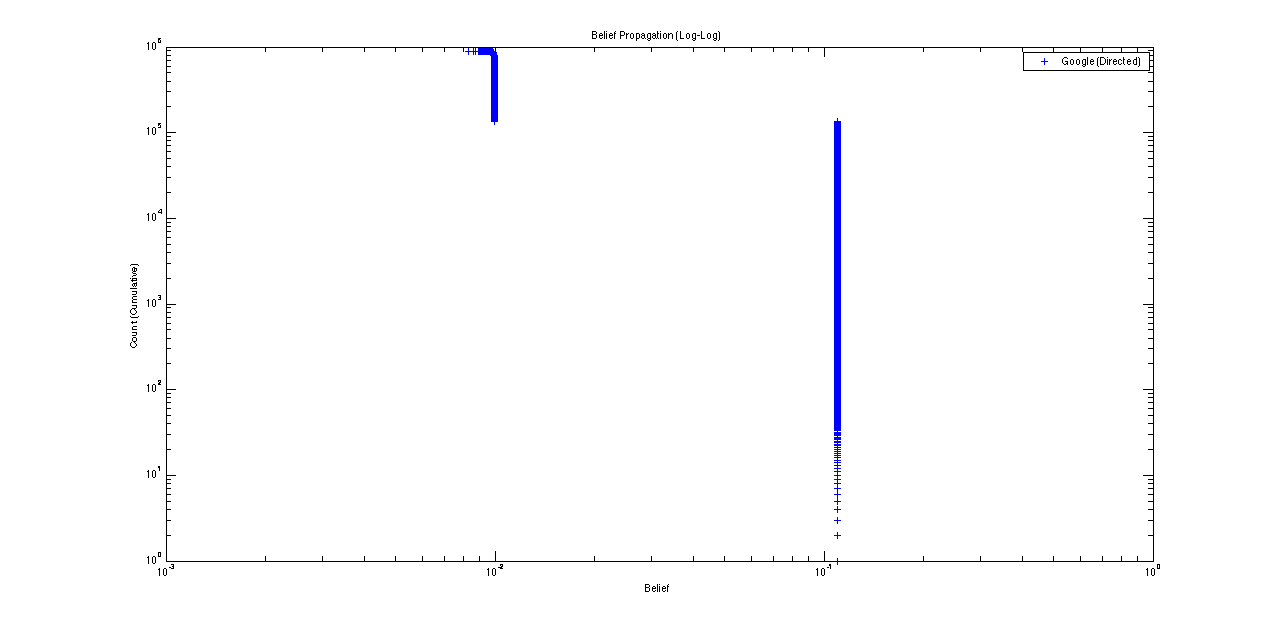
\includegraphics[width=\textwidth]{FIG/bp-google.png}
            \caption{Google}
            \label{fig:bp-google}
    \end{subfigure}
    ~ %add desired spacing between images, e. g. ~, \quad, \qquad etc.
      %(or a blank line to force the subfigure onto a new line)
    \begin{subfigure}[htbp]{0.9\textwidth}
            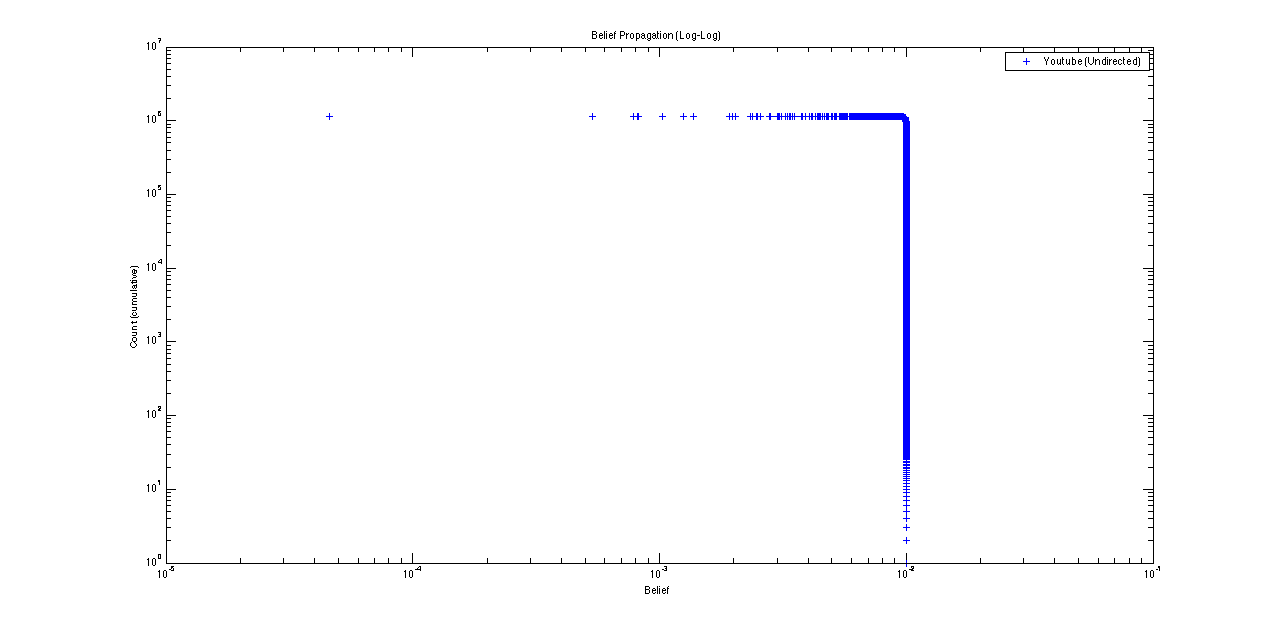
\includegraphics[width=\textwidth]{FIG/bp-youtube.png}
            \caption{Youtube}
            \label{fig:bp-youtube}
    \end{subfigure}
\end{figure} 

\addtocounter{figure}{-1}

\begin{figure} 
    \addtocounter{figure}{1}
    \centering 
        % ~ %add desired spacing between images, e. g. ~, \quad, \qquad etc.
          %(or a blank line to force the subfigure onto a new line)
        \begin{subfigure}[htbp]{0.9\textwidth}
                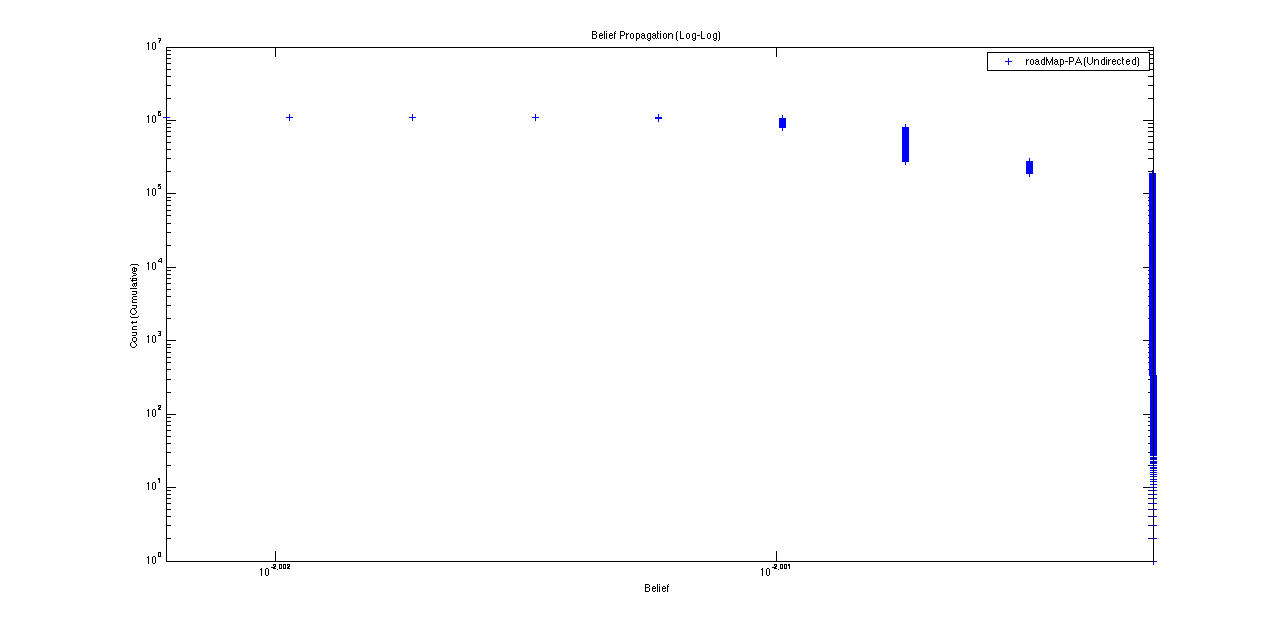
\includegraphics[width=\textwidth]{FIG/bp-pa.png}
                \caption{roadMap-PA}
                \label{fig:bp-pa}
        \end{subfigure}
        ~ %add desired spacing between images, e. g. ~, \quad, \qquad etc.
          %(or a blank line to force the subfigure onto a new line)
        \begin{subfigure}[htbp]{0.9\textwidth}
                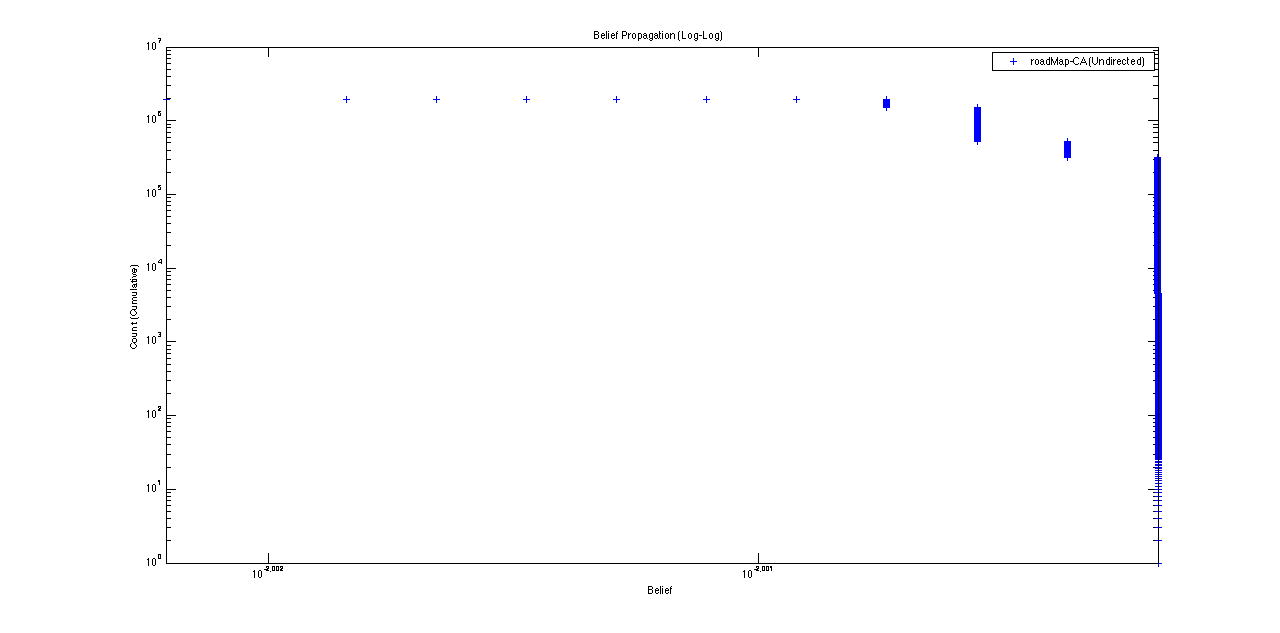
\includegraphics[width=\textwidth]{FIG/bp-ca.png}
                \caption{roadMap-CA}
                \label{fig:bp-ca}
        \end{subfigure}
        ~ %add desired spacing between images, e. g. ~, \quad, \qquad etc.
          %(or a blank line to force the subfigure onto a new line)
        \begin{subfigure}[htbp]{0.9\textwidth}
                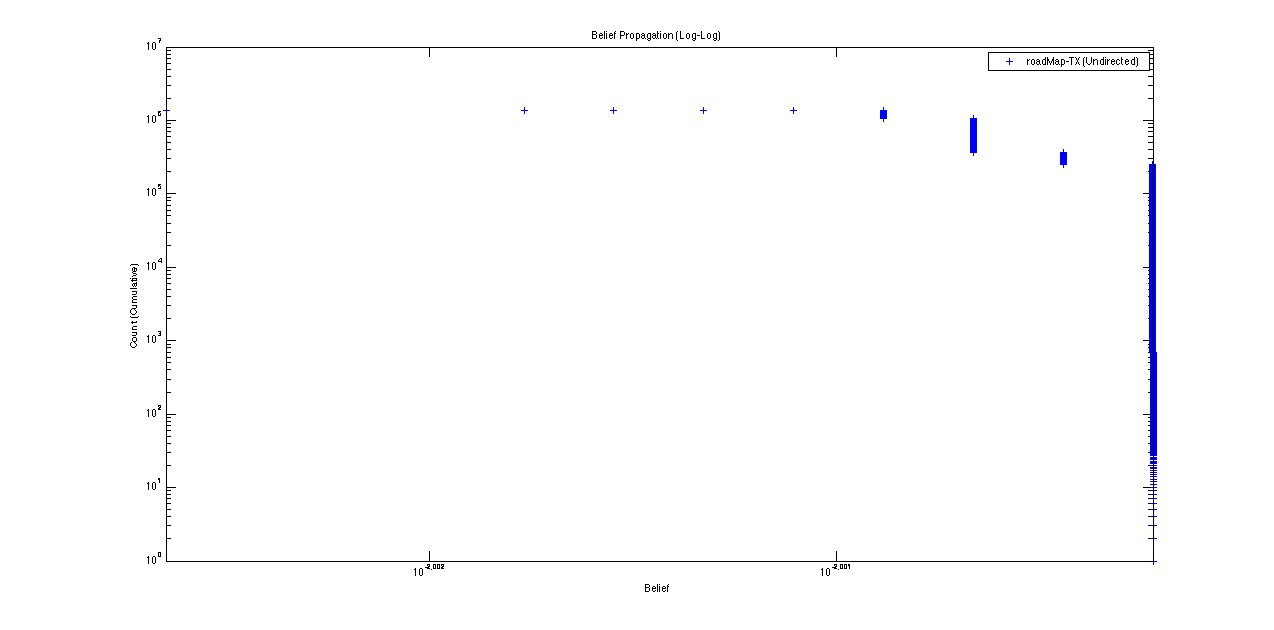
\includegraphics[width=\textwidth]{FIG/bp-tx.png}
                \caption{roadMap-TX}
                \label{fig:bp-tx}
        \end{subfigure}
        \caption{Belief Distribution}
        \label{fig:results6-1}
\end{figure}


%%%%%%%%%%%%%%%%%%%%%%%%%%%%%%%%%%%%%%%%%%%%%%%%%%%%%%%%%%%%%%%%%%%%%%%%%%%%%%%%%%
\subsection{Task 7: Count of Triangles}
\subsubsection{Accuracy Demonstration}
As we talked about in task 5, the eigenvalues calculated by Lanczos-SO are not all the eigenvalues of the adjacency matrix nor are the greatest values. As we do the experiment, the triangle counting are not accurate because of this. \\
The experiment result is as follow in Figure \ref{fig:results7}.\\
As can be seen by comparing the result of PostgreSQL implementation and MATLAB, the count of triangle has some difference. This is because the Lanczos algorithm we implemented failed to find out all the greatest eigenvalue. \\
But they all have the same pattern, that is, subject to the power law. There are a great many of nodes that have small number of triangle and a few number of nodes that have very large number of triangle.\\
From the computation from MATLAB, we can see that there are about 10 nodes with extremely large number of triangles, that maybe the super star on youtube website. \\
And there are stand out phenomenon at around triangle number 100. This may because there are certain youtube groups of people that they all know each other in the same group.

\begin{figure}
    \centering
    \begin{subfigure}[htbp]{0.8\textwidth}
            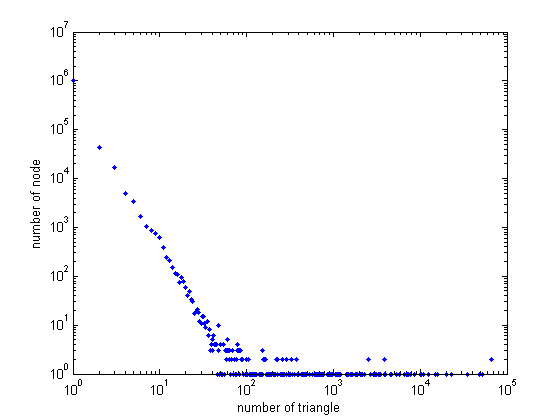
\includegraphics[width=\textwidth]{FIG/my_youtube_triangle.png}
            \caption{Youtube: Triangle Distribution}
            \label{fig:my_youtube_triangle}
    \end{subfigure}
    ~ %add desired spacing between images, e. g. ~, \quad, \qquad etc.
      %(or a blank line to force the subfigure onto a new line)
    \begin{subfigure}[htbp]{0.8\textwidth}
            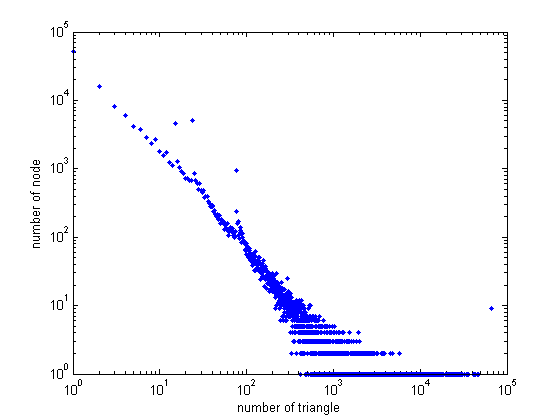
\includegraphics[width=\textwidth]{FIG/matlab_youtube_triangle.png}
            \caption{Youtube: Triangle Distribution(Matlab)}
            \label{fig:matlab}
    \end{subfigure}
    \caption{Weight/Triangle Distribution}
        \label{fig:results7}
\end{figure}

\subsubsection{Variety Demonstration}
We perform the test on 1M nodes social-Youtube dataset. From \ref{fig:results7}, we observes the ’triangle partic- ipation’ law (TPL).

%%%%%%%%%%%%%%%%%%%%%%%%%%%%%%%%%%%%%%%%%%%%%%%%%%%%%%%%%%%%%%%%%%%%%%%%%%%%%%%%%%
 \subsection{Task 8: Innovation Task}
 As we mentioned in the method section, we intend to extend algorithms to directed graph and weighted graph. As for directed graph, we have alread given the plot of web-Google graph in the variety sections of abbove related tasks. \\
 Here we will cover the case of weighted degree distribution and weighted PageRank distribution. The graph we use is Libimseti dataset.\\
 First we give the plot of in/out-degree and in/out weight as follows in Figure \ref{fig:results8}. \\
\begin{figure} 
    \centering 
        % ~ %add desired spacing between images, e. g. ~, \quad, \qquad etc.
          %(or a blank line to force the subfigure onto a new line)
        \begin{subfigure}[htbp]{0.6\textwidth}
                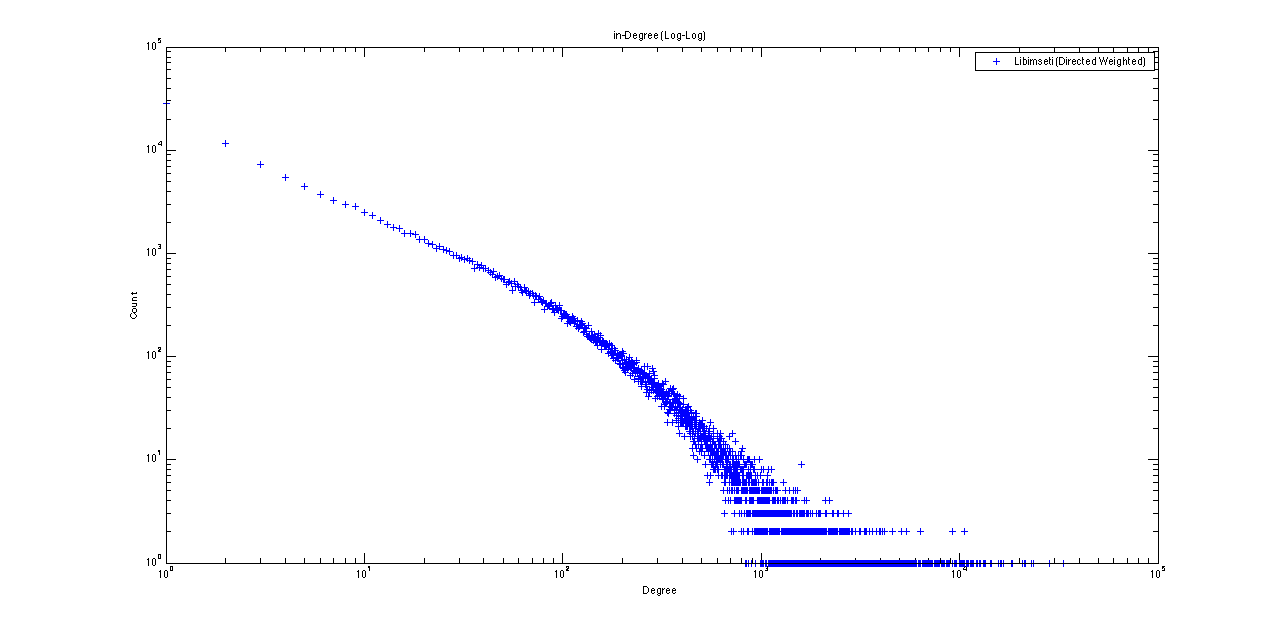
\includegraphics[width=\textwidth]{FIG/dw_ind.png}
                \caption{Libimseti in-Degree}
                \label{fig:dw_ind}
        \end{subfigure} %
        ~ %add desired spacing between images, e. g. ~, \quad, \qquad etc.
          %(or a blank line to force the subfigure onto a new line)
        \begin{subfigure}[htbp]{0.6\textwidth}
                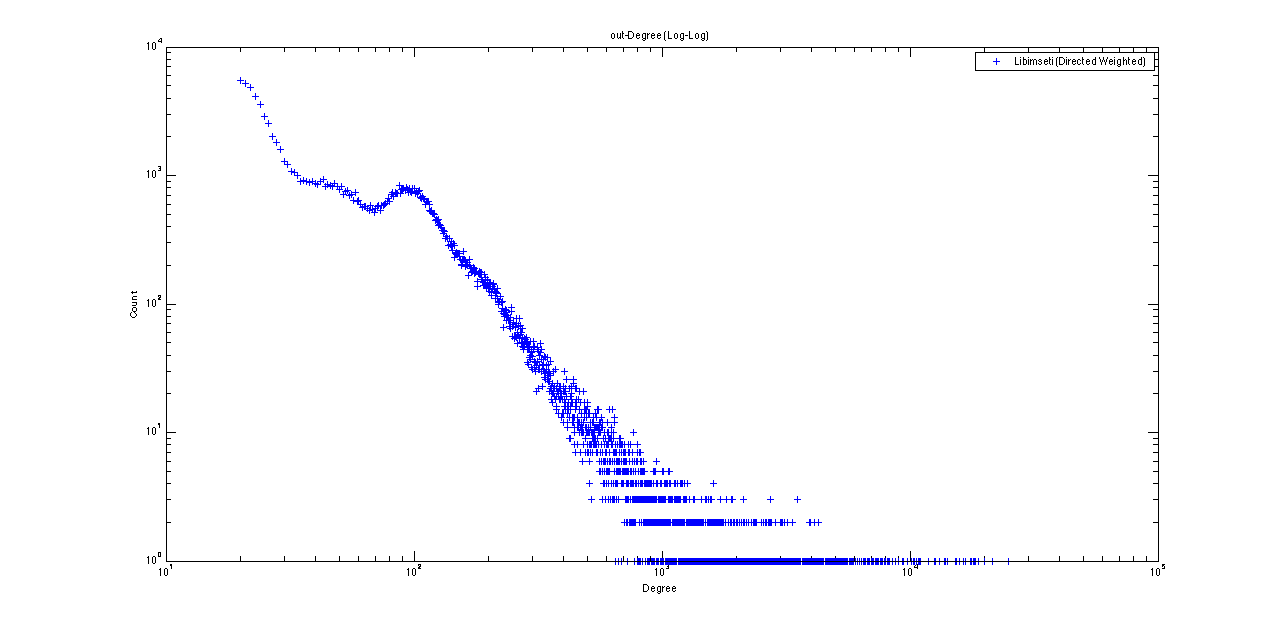
\includegraphics[width=\textwidth]{FIG/dw_outd.png}
                \caption{Libimseti out-Degree}
                \label{fig:dw_outd}
        \end{subfigure}
        ~ %add desired spacing between images, e. g. ~, \quad, \qquad etc.
          %(or a blank line to force the subfigure onto a new line)
        \begin{subfigure}[htbp]{0.6\textwidth}
                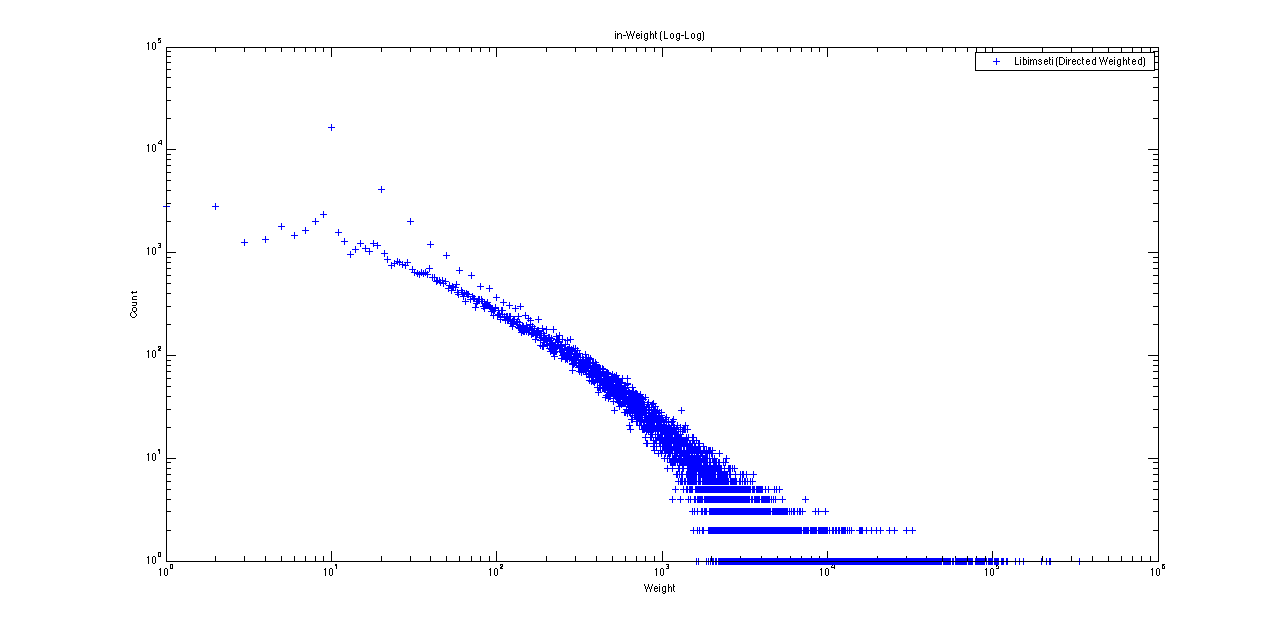
\includegraphics[width=\textwidth]{FIG/dw_inw.png}
                \caption{Libimseti in-Weight}
                \label{fig:dw_inw}
        \end{subfigure} %
        ~ %add desired spacing between images, e. g. ~, \quad, \qquad etc.
          %(or a blank line to force the subfigure onto a new line)
        \begin{subfigure}[htbp]{0.6\textwidth}
                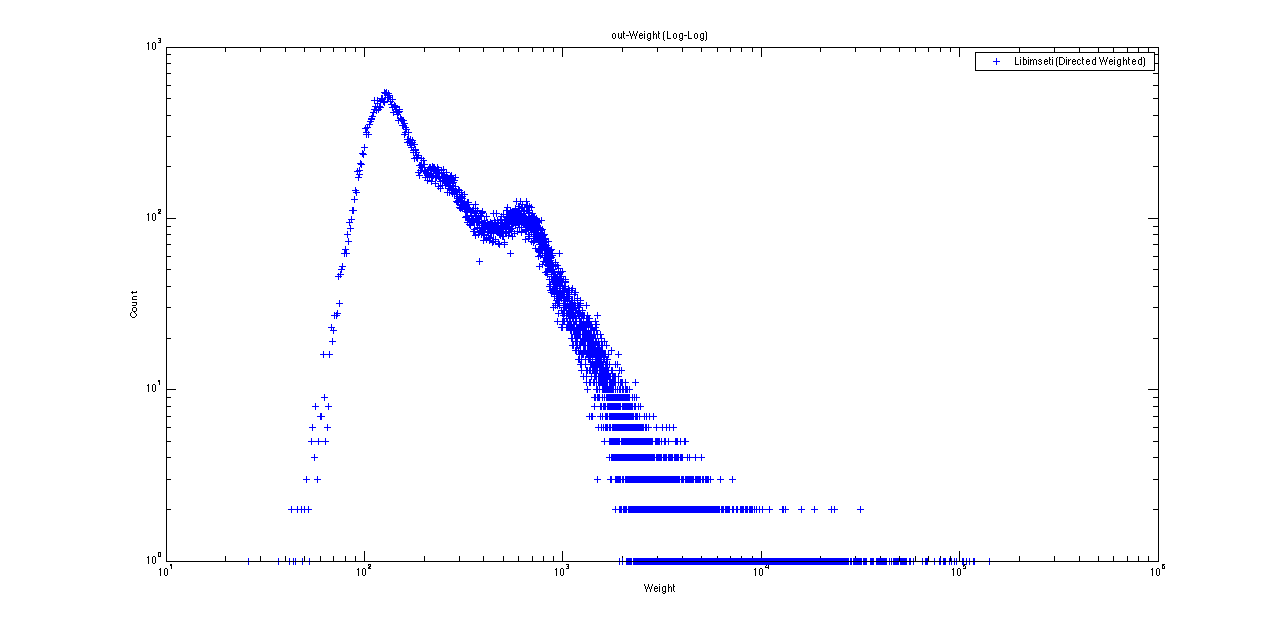
\includegraphics[width=\textwidth]{FIG/dw_outw.png}
                \caption{Libimseti out-Weight}
                \label{fig:dw_outw}
        \end{subfigure}
        \caption{Weight and Degree Distribution}
        \label{fig:results8}
\end{figure}
Then we plot in-weight and in-degree together as well as out-weight and out-degree together in Figure \ref{fig:results8-1}, which shows the SNAPSHOT POWER LAWS (SPL). \\

\begin{figure}
    \centering
    \begin{subfigure}[htbp]{0.8\textwidth}
            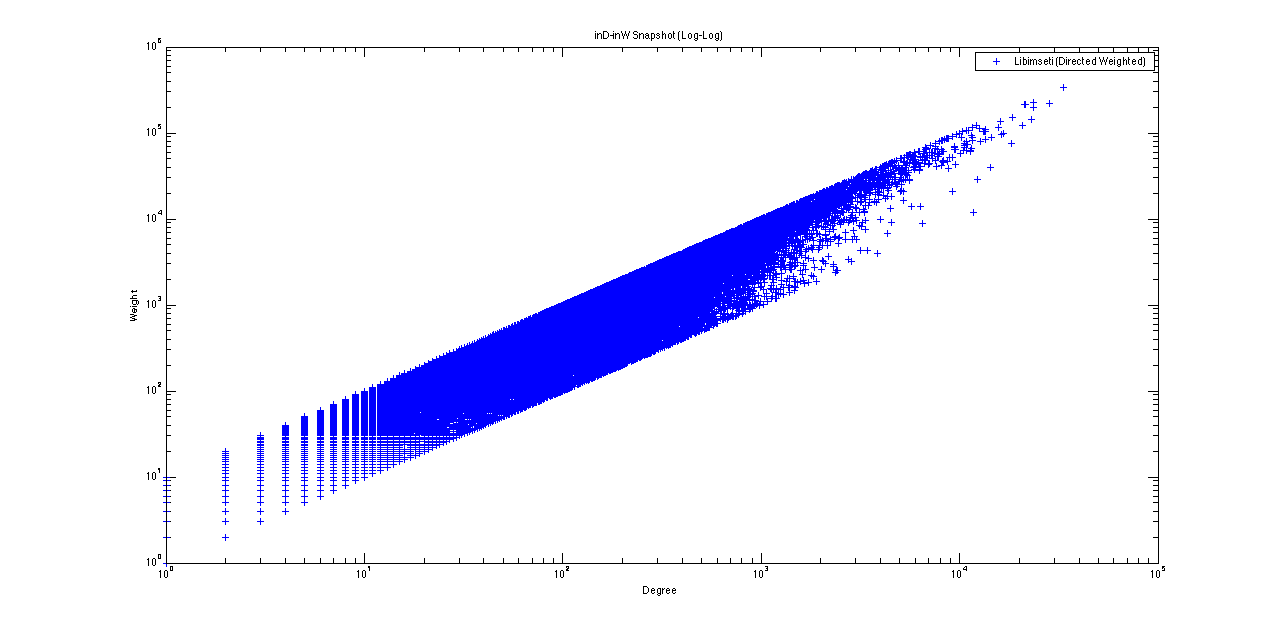
\includegraphics[width=\textwidth]{FIG/dw_in.png}
            \caption{inD-inW snapshot}
            \label{fig:dw-out}
    \end{subfigure}
    ~ %add desired spacing between images, e. g. ~, \quad, \qquad etc.
      %(or a blank line to force the subfigure onto a new line)
    \begin{subfigure}[htbp]{0.8\textwidth}
            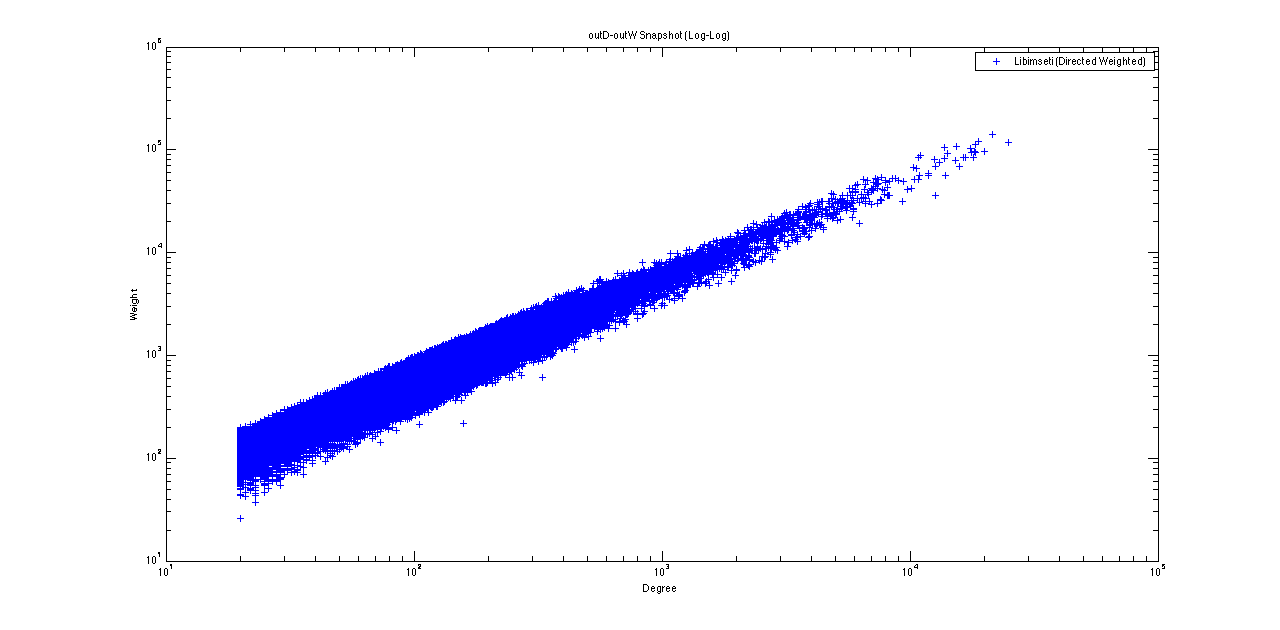
\includegraphics[width=\textwidth]{FIG/dw_out.png}
            \caption{outD-outW snapshot}
            \label{fig:dw-out}
    \end{subfigure}
    \caption{Weight/Degree Snapshot}
        \label{fig:results8-1}
\end{figure}

Finally, we give the plot of PageRank distribution and distributed PageRank distribution. From Figure \ref{fig:results8-2}, we can figure out that both of graphs follow the power law distribution and they are very similar to each other.
\begin{figure}
    \centering
    \begin{subfigure}[htbp]{0.8\textwidth}
            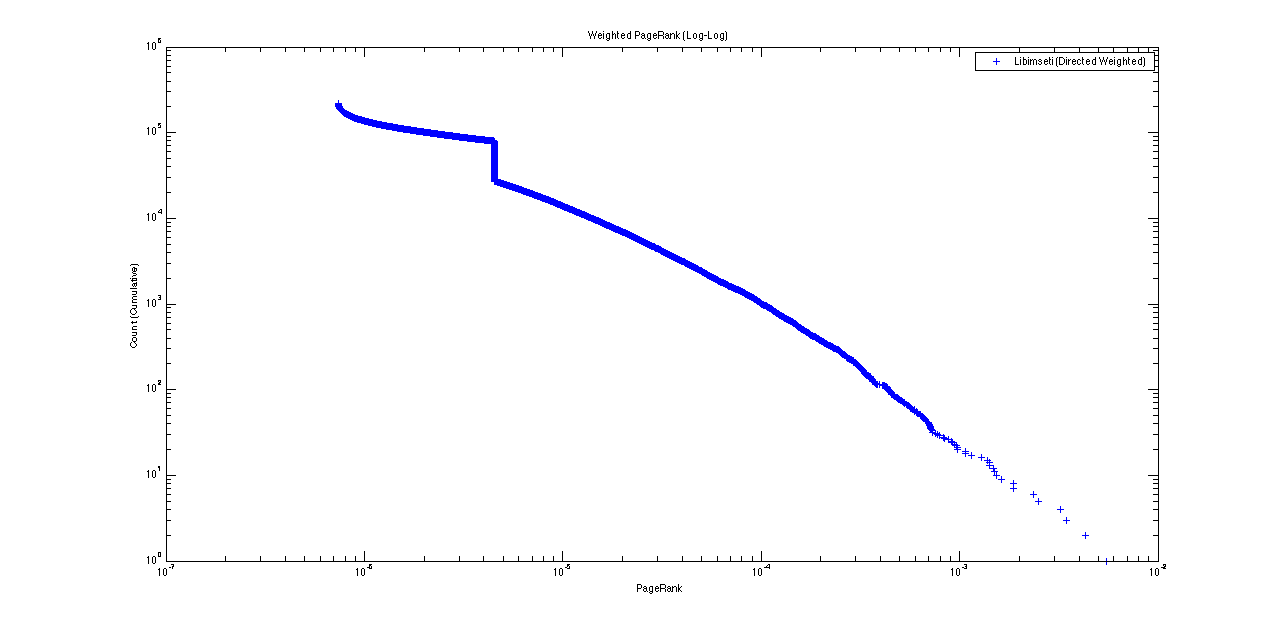
\includegraphics[width=\textwidth]{FIG/dw_pr.png}
            \caption{Weighted PageRank Distribution}
            \label{fig:dw-pr}
    \end{subfigure}
    ~ %add desired spacing between images, e. g. ~, \quad, \qquad etc.
      %(or a blank line to force the subfigure onto a new line)
    \begin{subfigure}[htbp]{0.8\textwidth}
            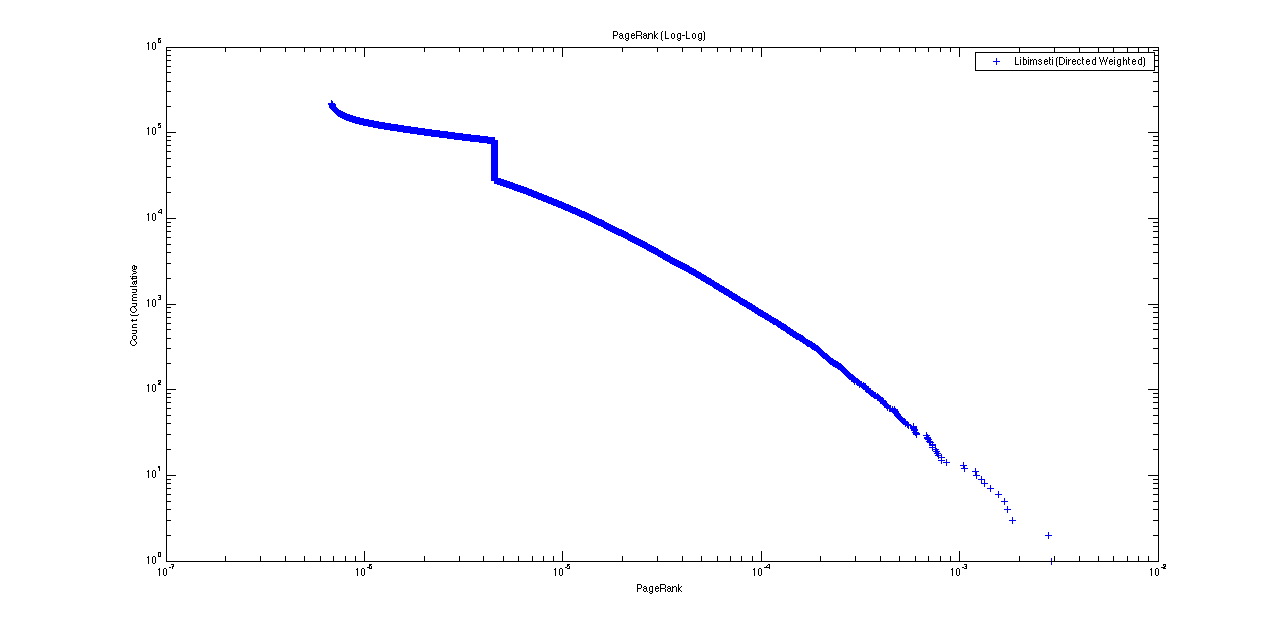
\includegraphics[width=\textwidth]{FIG/pr.png}
            \caption{PageRank Distribution}
            \label{fig:dw-pr2}
    \end{subfigure}
    \caption{PageRank vs Weighted PageRank}
        \label{fig:results8-2}
\end{figure}

\section{Conclusions}
    \label{sec:conclusions}
    In this report, we studied how to perform graphing mining in RDBMS.
Implementating graph queries using SQL has the following advantages:
\bit
\item it avoids the extra effort of extracting data and performing analysis elsewhere
\item it makes full use of the support of RDBMS(e.g. JOIN operations, data management, query optimization, etc.)
\eit
After performing graph mining on various large-scale dataset, we come to the conclusions: 
\bit
\item real world large graph data are skewed distributed, and thus power lawer distribution are applied at many places
\item large graph in information technology area such as graph social network and web graph behave very differently from real work network like road network in terms of small diameter
\eit


\bibliography{BIB/christosref,BIB/other,BIB/survey}
\bibliographystyle{plain}

\newpage
\appendix
\section{Appendix}

\subsection{Labor Division}

The team performed the following tasks:
\bit
\item Implementation of degree distribution [Emma, Fangyu]
\item Implementation of PageRank [Emma, Fangyu]
\item Implementation of (weakly) connected components [Emma, Fangyu]
\item Implementation of radius and diameter query [Emma]
\item Implementation of eigenvalues/singular values [Fangyu]
\item Implementation of Belief Propagation [Emma]
\item Implementation of Count of Triangles [Fangyu]
\item Experiments on the real data (Broad-spectrum graph mining) [Emma, Fangyu]
\item Innovation tasks [Emma, Fangyu]
\eit

A tentative progress plan for Emma Zhang:
\bit
\item by 10/10: Implementation of degree distribution [Done]
\item by 10/10: Implementation of PageRank [Done]
\item by 10/10: Implementation of (weakly) connected components [Done]
\item by 10/24: Implementation of radius and diameter query [Done]
\item by 10/24: Implementation of Belief Propagation [Done]
\item by 11/01: Broad-spectrum graph mining(phase 1) [Done]
\item by 11/07: Innovation task proposal [Done]
\item by 11/07: Progress Report Writing [Done]
\item by 11/21: Implementation of Innovation task [Done]
\item by 11/21: Broad-spectrum graph mining(phase 2) [Done]
\item by 11/26: Code Packaging and Final Report Writing [Done]
\eit

A tentative progress plan for Fangyu Gao:
\bit
\item 10/12-10/22: implement HEigen algorithm [Done]
\item 10/23-10/25: implement counting triangles algorithm [Done]
\item 10/26-11/01: implement counting triangles algorithm [Done]
\item 11/02-11/07: write progress report [Done]
\item 11/08-11/19: implement innovation projects [Done]
\item 11/20-11/26: Package code and write final report [Done]
\eit

\subsection{Full disclosure wrt dissertations/projects}

\paragraph{Emma Zhang:}
She is not doing any project or dissertation related to this project.
\paragraph{Fangyu Gao:} 
He is not doing any project or dissertation related to this project.

\subsection{Code Description}
One thing we insist on during our processing is the making the code we write to a software that is robustness and easy to use. \\
Therefore, we write functions using PL/pgSQL that defaultly comes with PostgresSQL. We break the tasks in our project into small pieces and write them in separate functions. This guarantee the reusable and readability of our software.\\
We use table name as input and output parameters when passing tables, this makes our codes easy to understand and convenient to use.
For example, the function “matrix\_multiply\_matrix” is in the following format:

matrix\_by\_matrix(dst\_matrix\_name, left\_matrix\_name, right\_matrix\_name) return void \\
If we want to calculate $A * B$ and put the result into C, that is $C = A * B$ we can use the statement:


matrix\_by\_matrix(C, A, B)\\
where A, B, C are the names of the three matrices. We always put the name of the return table in the first parameter of a function. This makes our software follow the usual coding style that output comes first(e.g. $C = A * B$). And by following this style, we make our functions easy to remember and convenient to use.\\
Table \ref{tab:func} lists the important functions we wrote have writen by now.

\begin{table}[htbf]
\begin{center} 
\begin{tabular}{|l | c | } \hline \hline 
Function name & Description \\ \hline
void matrix\_by\_matrix(A, B, C) & $A = B * C$ \\
void matrix\_by\_vector(a, A, b) & $a = A * b$ \\
void matrix\_transpose(A, B) & $A = B^T$ \\
double vector\_by\_vector(a, b) & $a^T * b$ \\
void vector\_scale(a, b, lambda) & $a = lambda * b$ \\ \hline
\end{tabular} 
\end{center} 
\caption{Basic Functions}
\label{tab:func} 
 \end{table}

\newpage
\pagenumbering{roman}
\tableofcontents


\end{document}
